\subsection{Optimization for Inference}

\begin{frame}{Introduction}
    \textbf{Inspiration from previous algorithms:}
\begin{itemize}
    \item The previous Algorithms~\ref{alg:sum-product-variable-elimination} and~\ref{alg:clique-tree-variable-elimination} directly produce posterior distributions.
    \begin{itemize}
        \pause \item Either in terms of factors or in terms of messages.
    \end{itemize}
    \pause \item \underline{Problem:} What should we do when clique tree has prohibitively large cliques?
    \pause \item \underline{Technical insight:} The calibration conditions~\eqref{eq:calibrated-beliefs} give us an idea of how to iteratively improve our beliefs, even if the cluster graph we operate on is not a clique tree.
\end{itemize}
\pause
\textbf{General Ideas for inference for arbitrary graphs:}
\begin{itemize}
    \pause \item Use clique tree message passing on cluster graphs other than trees that might have smaller cliques.
    \begin{itemize}
        \pause \item Loopy belief propagation.
    \end{itemize}
    \pause \item Use message passing on clique trees with approximate messages.
    \begin{itemize}
        \pause \item Expectation propagation.
    \end{itemize}
    \pause \item Solve exactly an approximation of the original probability distribution.
    \begin{itemize}
        \pause \item Mean field methods.
    \end{itemize}
\end{itemize}
\pause
\textbf{Viewpoints:}
\begin{itemize}
    \pause\item \underline{Procedural:} Look at an algorithm in terms of its operations.
\begin{itemize}
\pause \item Analoguous to sum-product variable elimination Algorithm~\ref{alg:sum-product-variable-elimination}.
\end{itemize}
\pause \item \underline{Optimization:} Search for a set of conditions to be satisfied.
\begin{itemize}
\pause \item Analoguous to clique-tree message passing Algorithm~\ref{alg:calibration-sum-product-clique-tree} and the calibration equations~\eqref{eq:calibrated-beliefs}.
\end{itemize}
\end{itemize}
\end{frame}

\begin{frame}{Preliminaries}
    \begin{itemize}
    \item First, a few stochastic preliminaries are needed.
    \item We want to measure how close two probability distributions are for optimization. For this we will use entropy.
    \end{itemize}
    \pause
    \begin{definition}[Relative Entropy]
        The relative entropy betwen two probability distributions $\Pb_1$ and $\Pb_2$ is defined as
        \begin{equation}
            D(\Pb_1 || \Pb_2) = \E_{\Pb_1}[\log(\frac{\Pb_1}{\Pb_2})] = \sum_{x \in \mathcal{X}} \Pb_1[x] \log( \frac{\Pb_1[x]}{\Pb_2[x]})\,.
        \end{equation}
    \end{definition}
    \pause
    \begin{proposition}
       The relative entropy is non-negative and zero iff $\Pb_1 = \Pb_2$. 
    \end{proposition}
    \pause
    \begin{itemize}
        \item However, $D$ is not symmetric, i.e.\ $D(\Pb_1 || \Pb_2) \neq D(\Pb_2 || \Pb_1)$ in general.
    \end{itemize}
    \pause
    \begin{itemize}
        \item We will also use the entropy of a probability distribution for favoring distributions that are ``as random as possible'' later on.
    \end{itemize}
    \pause
    \begin{definition}[Entropy]
        The entropy of a probability distribution $\Pb$ is defined as
        \begin{equation}
            H(\Pb) = -\E_{\Pb}[\log(\Pb)] = -\sum_{x \in \mathcal{X}} \Pb[x] \log(\Pb[x])\,.
        \end{equation}
    \end{definition}
\end{frame}

\begin{frame}{Inference as Optimization}
    \textbf{Optimization for inference idea:}
    \begin{itemize}
        \item Search over a set of beliefs $Q(\mathcal{X}) = \frac{\prod_i \beta_i}{\prod_{ij} \mu_{ij}}$ that is close to $\Pb$ w.r.t.\ $D$.
        \pause \item Recall that beliefs, when calibrated, must satisfy $\beta_i(C_i) = Q(C_i)$ and $\mu_{ij}(C_i \cap C_j) = Q(C_i \cap C_j)$.
        \pause\item Let $T$ be a cluster graph, then directly searching over beliefs for doing inference can be cast as:
    \end{itemize}
    \pause
    \begin{equation}
    \begin{aligned}
            \min_Q\  & D(Q || \Pb_{\Phi}) \\
            \text{subject to } & \mu_{ij}(s_{ij}) = \sum_{c_i: c_{i|S_{ij}} = s_{ij}} \beta_i(c_i) \quad \forall ij, s_{ij} \\
            & \sum_{c_i} \beta_i(c_i) = 1
    \end{aligned}
    \end{equation}
    \pause
    \begin{corollary}
        If $T$ is a clique tree, we obtain the calibration equations~\eqref{eq:calibrated-beliefs} and thus posterior distributions.
    \end{corollary}
    \pause
    \begin{itemize}
    \item Evaluating $D(Q || \Pb_{\Phi})$ is intractable in general. Hence, the above formulation is a conceptual starting point that does not immediately yield a practical algorithm.
    \end{itemize}
\end{frame}

\begin{frame}{Energy Functional}
    \begin{definition}[Energy Functional]
    Define the energy functional as
    \begin{equation}
        F[\tilde{\Pb}_{\Phi},Q] = \E_Q[\log(\tilde{\Pb}[\mathcal{X}])]  + H_Q(\mathcal{X}) = \sum_{\phi \in \Phi} \E_Q[\log(\phi)] + H_Q(\mathcal{X})
    \end{equation}
    \end{definition}
\pause
    \begin{theorem}
    \label{thm:energy-functional}
    \begin{equation}
        D(Q || \Pb_{\Phi}) = \log(Z) - F[\tilde{\Pb}_{\Phi},Q]\,.
    \end{equation}
    \end{theorem}
\pause
    \begin{proof}
        First, by decomposing the relative entropy we get
        %\begin{equation}
            $
            D(Q || \Pb_{\Phi}) = \E_Q[\log(Q(\mathcal{X}))] - \E_Q[\log(\tilde{\Pb}_{\Phi}(\mathcal{X}))]
            $.
        %\end{equation}
\pause
        Using the product form of the Gibbs distribution gives
        %\begin{equation}
            $
            \log(\Pb_{\Phi}(\mathcal{X})) = \sum_{\phi \in \Phi} \phi(\mathcal{X}_{\Scope[\phi]}) - \log(Z)
        $.
        %\end{equation}
\pause
        Plugging the definition of the entropy $H_Q(\mathcal{X})$ into the first term yields
        \begin{equation}
            D(Q || \Pb_{\Phi}) = -H_Q(\mathcal{X}) - \E_{Q}\left[ \sum_{\phi \in \Phi} \log(\phi(\mathcal{X}_{\Scope[\phi]})) \right] + \E_Q[\log(Z)] = -F[\tilde{\Pb}_{\Phi},Q] + \log(Z)\,.
        \end{equation}
    \end{proof}
\end{frame}

\begin{frame}{Energy Functional}
    \begin{itemize}
    \item The free energy is more amenable to optimization:
    \begin{itemize}
\pause
        \item The first term $\E_Q[\log(\tilde{\Pb}_{\Phi}(\mathcal{X}))]$ factorizes according to the involved factors, splitting into smaller sums.
\pause
        \item The second term $H_Q(\mathcal{X})$ might be amenable depending on the choice of the potential family of possible $Q$'s.
    \end{itemize}
\pause
    \item The term $\log(Z)$ is not accounted for in the free energy and remains hard to compute. However, since $D \geq 0$, we have
    \begin{equation}
        \log(Z) \geq F[\tilde{\Pb}_{\Phi},Q]\,.
    \end{equation}
\pause
    \begin{itemize}
        \item If $D(Q || \Pb_{\Phi})$ is small, then we have a good approximation to $Z$.
    \end{itemize}
\pause
    \item Thus, we will investigate optimizing the free energy as
    \end{itemize}
    \begin{equation}
        \label{eq:free-energy-optimization}
    \begin{aligned}
        \max_Q\ & F[\tilde{\Pb}_{\Phi},Q] \\
        \text{subject to } & \mu_{ij}(s_{ij}) = \sum_{c_i: c_{i|S_{ij}} = s_{ij}} \beta_i(c_i) \quad \forall ij, s_{ij} \\
        & \sum_{c_i} \beta_i(c_i) = 1 \quad \forall i\\
        & \beta_i(c_i) \geq 0 \quad \forall i, c_i \\
    \end{aligned}
    \end{equation}
\end{frame}

\begin{frame}{Factored Free Energy Functional}
\begin{itemize}
    \item As noted above, the entropy might be hard to compute.
    \pause \item An approximation that factorizes over the cluster structure of $T$ is
\end{itemize}
\pause
\begin{definition}
   Let $T$ be a cluster tree, Q a set of beliefs and $\xi$ an assignment that maps factors to clusters in $T$. 
   Let $\psi_i = \prod_{\phi: \xi(\phi) = i} \phi$ be the product of all factors in cluster $i$.
   Then the factored free energy is defined as
\begin{equation}
        \tilde{F}[\tilde{\Pb}_{\Phi},Q] = \sum_{\phi \in \Phi} \E_{C_i \sim \beta_i}[\log(\psi_i)] + \sum_{C_i} H_{\beta_i}(C_i) - \sum_{ij} H_{\mu_{ij}}(_{ij}) 
\end{equation}
\end{definition}
\pause
\begin{theorem}[Factored Free Energy = Free Energy for calibrated beliefs \& cluster trees]
    \label{thm:factored-equals-free-energy}
    Let $T$ be a cluster tree and let $\beta$ be calibrated.
    Then $\tilde{F}[\tilde{\Pb}_{\Phi},Q] = F[\tilde{\Pb}_{\Phi},Q]$.
\end{theorem}
\pause
\begin{proof}
    Since $\beta_i(c_i) = Q(c_i)$ we have $\sum_i \E_{C_i \sum \beta_i}[\log(\psi_i)] = \sum_{\phi \in \Phi} \E_Q[\log(\phi)]$.
    \pause
    It remains to show $H_Q(\mathcal{X}) = \sum_{i} H_{\beta_i}(C_i) - \sum_{ij}  H_{\mu_{ij}}(S_{ij})$.
    \pause
    This equality follows directly from the definition $Q(\mathcal{X}) = \frac{\prod_i \beta_i}{\prod_{ij} \mu_{ij}}$ and Theorem~\ref{thm:calibrated-clique-tree-Q}.
\end{proof}
\end{frame}

\begin{frame}{Factored Free Energy Optimization}
\begin{itemize}
    \item With the help of Theorem~\ref{thm:factored-equals-free-energy} we can reformulate the harder problem~\eqref{eq:free-energy-optimization} as a simpler one by replacing $F$ with $\tilde{F}$ in~\eqref{eq:free-energy-optimization}.
\begin{equation}
    \label{eq:factored-free-energy-optimization}
    \max_{\beta,\mu} \tilde{F}[\tilde{\Pb}_{\Phi}, Q] \quad\text{ s.t. }\quad \mu_{ij} = \sum_{C_i \backslash S_{ij}} \beta_i,\quad \sum_{C_i} \beta_i(C_i) = 1,\quad \beta_i \geq 0\,.
\end{equation}
\pause
    \item When we optimize~\eqref{eq:factored-free-energy-optimization} we will not get to the global optimum in general for non-tree clique graphs.
     \begin{itemize}
        \pause \item Instead, the attainable stationary points, e.g.\ $\nabla \tilde{F} = 0$, will be characterized by a set of equations.
    \end{itemize}
 \end{itemize}
 \pause
 \begin{theorem}[Stationary Points of~\eqref{eq:factored-free-energy-optimization}]
    \label{thm:stationary-points-factored-free-energy}
 A set of beliefs $Q$ is a stationary point of~\eqref{eq:factored-free-energy-optimization} iff there exists a set of factors $\{\delta_{i \rightarrow j}[S_{ij}] : ij \in E_T\}$ such that
 \begin{equation}
    \delta_{i \rightarrow j} \propto \sum_{C_i \backslash S_{ij}} \psi_i \cdot \prod_{k \in \Nb(i) \backslash \{j\}} \delta_{k \rightarrow i}
 \end{equation}
 \pause
 In this case we have 
 \begin{equation}
 \beta_i \propto \psi \cdot \prod_{j \in \Nb(i)} \delta_{j \rightarrow i}
 \end{equation}
 \pause
 \begin{equation}
 \mu_{ij} = \delta_{i \rightarrow j} \delta_{j \rightarrow i}\,.
 \end{equation}
 \end{theorem}
\end{frame}

\begin{frame}{Proof of Factored Free Energy Fixed Points}
    \begin{proof}
       First, we write the Lagrangian of~\eqref{eq:factored-free-energy-optimization} w.r.t.\ the two equality constraints as 
       \begin{equation}
        J(\beta,\mu,\lambda) = \tilde{F}[\tilde{\Pb}_{\Phi},Q]
        \pause
        - \sum_i \lambda_i \underbrace{\left( \sum_{C_i} \beta_i - 1 \right)}_{\sum_{c_i} \beta_i(c_i) = 1}
        \pause
        - \sum_{ij} \sum_{s_{ij}}\lambda_{i \rightarrow j}(s_{ij}) \underbrace{\left( \sum_{c_i \sim s_{ij}} \beta_i(c_i) - \mu_{ij}(s_{ij}) \right)}_{\mu_{ij}(s_{ij}) = \sum_{c_i \sim s_{ij}} \beta_i(c_i)}
       \end{equation}
       \pause
    Then
    \begin{equation}
        \frac{\partial J}{\partial_{\beta_i(c_i)}} = \log(\psi_i(c_i)) - \log(\beta_i(c_i)) - 1 - \lambda_i - \sum_{j \in \Nb(i)} \lambda_{i \rightarrow j}(s_{ij}) \,.
    \end{equation}
    \pause
    \begin{equation}
        \frac{\partial J}{\partial_{\mu_{ij}(s_{ij})}} = \log(\mu_{ij}(s_{ij})) + 1 + \lambda_{i \rightarrow j}(s_{ij}) + \lambda_{j \rightarrow i}(s_{ij}) \,.
    \end{equation}
    \pause
    For stationary points these derivatives are zero. Setting to zero, rearranging and exponentiating gives
    \pause
    \begin{equation}
        \beta_i(c_i) = \exp(-1-\lambda_i) \psi_i(c_i) \prod_{j \in \Nb(i)} \exp{-\lambda_{i \rightarrow j}(s_{ij})} \,.
    \end{equation}
    \pause
    \begin{equation}
        \label{eq:mu-exp-lambda}
        \mu_{ij}(s_{ij}) = \exp(-1) \exp(-\lambda_{i \rightarrow j}(s_{ij})) \exp(-\lambda_{j \rightarrow i}(s_{ij})) \,.
    \end{equation}
\end{proof}
\end{frame}

\begin{frame}{Proof cont.\ of Factored Free Energy Fixed Points}
    \begin{proof}
    By observing the similarity of~\eqref{eq:mu-exp-lambda} and the equality $\mu_{ij} = \delta_{i \rightarrow j} \delta_{j \rightarrow i}$ we define
    \begin{equation}
        \delta_{i \rightarrow j}(s_{ij}) = \exp( - \lambda_{i \rightarrow j}(s_{ij}) - 0.5) \,.
    \end{equation}
    \pause 
We can rewrite $\beta$ and $\mu$ from above as
    \begin{equation}
        \beta_i(c_i) = \exp\left(-1-\lambda_i + \frac{1}{2} \abs{\Nb(i)}\right) \psi_i(c_i) \prod_{j \in \Nb(i)} \delta_{j \rightarrow i}(s_{ij})\,.
    \end{equation}
    \pause
    \begin{equation}
        \mu_{ij}(s_{ij}) = \delta_{j \rightarrow i}(s_{ij}) \delta_{i \rightarrow j}(s_{ij})\,.
    \end{equation}
    \pause
    Combining gives
    \begin{multline}
       \delta_{i \rightarrow j}(s_{ij}) = \frac{\mu_{ij}(s_{ij})}{\delta_{j \rightarrow i}(s_{ij})} 
       \pause = \frac{\sum_{c_i \sim s_{ij}} \beta_i(c_i)}{\delta_{j \rightarrow i}(s_{ij})} \\
       \pause = \exp\left( -\lambda_i - 1 + \frac{1}{2} \abs{\Nb(i)} \right) \sum_{c_i \sim s_{ij}} \psi_i(c_i) \prod_{k \in \Nb(i) \backslash \{j\}} \delta_{k \rightarrow i}(s_{ij})\,.
    \end{multline}
    \end{proof}
\end{frame}

%\begin{frame}{Cluster-Graph Belief Propagation}
%    \begin{itemize}
%        \item We defined clique trees as cluster graphs that 
%        \begin{itemize}
%            \pause \item are trees
%            \pause \item have the running intersection property.
%        \end{itemize}
%        \pause \item Our plan: Remove tree condition, generalize rip, see what we can do with message passing.
%    \end{itemize}
%    \pause
%    \begin{definition}[RIP for Cluster Graphs]
%        We say that a cluster graph $U$ satisfies the running intersection property if for all variables $X$ such that $X \in C_i$ and $X \in C_j$ there is a single path between $C_i$ and $C_j$ for which $X \in S_e$ for all edges $e$ in the path.
%    \end{definition}
%    \begin{itemize}
%    \pause \item Obviously reverts to clique tree rip for clique trees.
%    \pause \item All edges with $X$ in them form a tree that span all clusters containing $X$.
%    \pause \item There is a single path through which information directly containing $X$ can flow through.
%    \begin{itemize}
%        \pause \item Prevents information about $X$ to ``cycle'' through the graph for belief propagation.
%    \end{itemize}
%    \end{itemize}
%    \pause
%    \begin{definition}[Cluster Graph Calibration]
%        \label{def:cluster-graph-calibration}
%        We say that a cluster graph is calibrated if for each edge $ij$ we have that
%        \begin{equation}
%            \sum_{C_i \backslash S_{ij}} \beta_i = \sum_{C_j \backslash S_{ij}} \beta_j\,.
%        \end{equation}
%    \end{definition}
%    \begin{itemize}
%    \pause \item Definition~\ref{def:cluster-graph-calibration} might be weaker than Definition~\ref{def:calibrated-messages} for clique trees when the sepsets do not contain all joint variables.
%    \end{itemize}
%\end{frame}

\begin{frame}{Asynchronous Sum-Product Message Passing in Cluster Graph}
    \textbf{Idea:} Theorem~\ref{thm:stationary-points-factored-free-energy} suggests to chase messages such that $\delta_{i \rightarrow j} \propto \sum_{C_i \backslash S_{ij}} \psi_i \cdot \prod_{k \in \Nb(i) \backslash \{j\}} \delta_{k \rightarrow i}$.
    \pause
    \begin{itemize}
        \item Asynchronous BP: Try to make messages fulfill stationarity conditions one after the other.
    \end{itemize}
    \pause
    \begin{minipage}{0.6\textwidth}
\begin{algorithm}[H]
    \caption{Asynchronous Sum-Product Message Passing in Cluster Graph}
    \label{alg:asynchronous-spmp}
    \KwInput{factors $\Phi$, cluster graph $U$, step size $\alpha$, factor-cluster assignment $\xi$}
    \tcp{Initialize Cluster Graph}
    \For{each cluster $C_i$}
    {
        $\psi_i = \prod_{\phi: \xi(\phi) = i} \phi$\;
    }
    \pause
    \For{each edge $ij$}
    {
        $\delta_{i \rightarrow j} \leftarrow 1$, $\delta_{j \rightarrow i} \leftarrow 1$\;
    }
    \pause
    \tcp{Message Passing}
    \While{not converged}
    {
        Select $i \rightarrow j$\;
        \pause
        \tcp{SP-Message(i,j)}
        $\delta'_{i \rightarrow j} \leftarrow \sum_{C_i \backslash S_{ij}} \psi_i \cdot \prod_{k \in \Nb(i) \backslash \{j\}} \delta_{k \rightarrow i}$\;
        \pause
        \tcp{Make damped message update step}
        $\delta_{i \rightarrow j} \leftarrow \alpha \cdot \delta'_{i \rightarrow j} + (1-\alpha) \delta_{i \rightarrow j}$\;
    }
    \pause
    \tcp{Compute Beliefs}
    \For{each clique $i$}
    {
        $\beta_i \leftarrow \psi_i \cdot \prod_{j \in \Nb(i)} \delta_{j \rightarrow i}$\;
    }
\end{algorithm}
\end{minipage}
    \begin{minipage}{0.39\textwidth}
\begin{itemize}
    \pause \item Other than $U$ being a graph, Algorithm~\ref{alg:asynchronous-spmp} is almost identical to Algorithm~\ref{alg:calibration-sum-product-clique-tree}.
    \pause \item But message passing schedule is unclear, hot to select $ij$, how to generalize ``ready to transmit''?
    \begin{itemize}
        \pause \item For a cycle there is no cluster that has received all incoming messages!
    \end{itemize}
    \pause \item Messages for next iteration are convex combination of sum-product update and previous messages
    \pause \item In practice asynchronous with $\alpha = 1$ might oscillate: Beliefs cyclically change value
    \begin{itemize}
        \pause \item $\alpha < 1$ often necessary for convergence.
    \end{itemize}
\end{itemize}
\end{minipage}
\end{frame}

\begin{frame}{Synchronous (Parallel) Sum-Product Message Passing in Cluster Graph}
    \textbf{Idea:} Theorem~\ref{thm:stationary-points-factored-free-energy} suggests to chase messages such that $\delta_{i \rightarrow j} \propto \sum_{C_i \backslash S_{ij}} \psi_i \cdot \prod_{k \in \Nb(i) \backslash \{j\}} \delta_{k \rightarrow i}$.
    \pause
    \begin{itemize}
        \item Synchronous BP: Try to make messages fulfill stationarity conditions all at once.
    \end{itemize}
    \begin{minipage}{0.6\textwidth}
\begin{algorithm}[H]
    \caption{Synchronous Sum-Product Message Passing in Cluster Graph}
    \label{alg:synchronous-spmp}
    \KwInput{factors $\Phi$, cluster graph $U$, step size $\alpha$, factor-cluster assignment $\xi$}
    \For{each cluster $C_i$} 
    {
        $\psi_i = \prod_{\phi: \xi(\phi) = i} \phi$\;
    }
    \pause
    \For{each edge $ij$}
    {
        $\delta_{i \rightarrow j} \leftarrow 1$, $\delta_{j \rightarrow i} \leftarrow 1$\;
    }
    \pause
    \tcp{Message Passing}
    \While{not converged}
    {
        \tcp{Compute sum-product message}
        \For{each $i \rightarrow j$}
        {
            $\delta'_{i \rightarrow j} \leftarrow \sum_{C_i \backslash S_{ij}} \psi_i \cdot \prod_{k \in \Nb(i) \backslash \{j\}} \delta_{k \rightarrow i}$\;
        }
        \pause
        \tcp{Make damped message update step}
        \For{each $i \rightarrow j$}
        {
            $\delta_{i \rightarrow j} \leftarrow \alpha \cdot \delta'_{i \rightarrow j} + (1-\alpha) \cdot \delta_{i \rightarrow j}$\;
        }
    }
    \pause
    \tcp{Compute Beliefs}
    \For{each clique $i$}
    {
        $\beta_i \leftarrow \psi_i \cdot \prod_{j \in \Nb(i)} \delta_{j \rightarrow i}$\;
    }
\end{algorithm}
\end{minipage}
    \begin{minipage}{0.39\textwidth}
        \begin{itemize}
            \pause \item All message updates are computed in parallel.
            \begin{itemize}
                \pause \item No message passing schedule necessary.
            \end{itemize}
            \pause \item Asynchronous message passing typically significantly better than synchronous message passing.
            \begin{itemize}
                \pause \item But synchronous message passing has parallelization potential.
            \end{itemize}
        \end{itemize}
\end{minipage}
\end{frame}

\begin{frame}{Cluster Graph Reparametrization}
    \begin{theorem}
        Let $U$ be a cluster graph over $\Phi$. Consider beliefs $\beta_i$ and sepsets $\mu_{ij}$ at any iteration of Algorithm~\ref{alg:asynchronous-spmp}~or~\ref{alg:synchronous-spmp}.
        Then
        \begin{equation}
            \tilde{\Pb}_{\Phi}[\mathcal{X}] = \frac{\prod_i \beta_i(C_i)}{\prod_{ij} \mu_{ij}(S_{ij})}\,.
        \end{equation}
    \end{theorem}
    \pause
    \begin{proof}
        Recall that $\beta_i = \psi_i \prod_{j \in \Nb(i)} \delta_{j \rightarrow i}$ and $\mu_{ij} = \delta_{i \rightarrow j} \delta_{j \rightarrow i}$.
        \pause
        Then
        \begin{equation}
           \frac{\prod_i \beta_i(C_i)}{\prod_{ij} \mu_{ij}(S_{ij})} 
           \pause= \frac{\prod_i \psi_i \prod_{j \in \Nb(i)} \delta_{j \rightarrow i}}{\prod_{ij} \delta_{i \rightarrow j} \delta_{j \rightarrow i}}
           \pause = \prod_{i} \psi_i(C_i) 
           \pause = \prod_{\phi \in \Phi} \phi
        \end{equation}
    \end{proof}
\end{frame}


\begin{frame}{Sum-Product Message Passing Considerations}
\begin{minipage}[t]{0.6\textwidth}
    \textbf{Information Propagation:}
    \begin{itemize}
        \item Assume cluster graph has diameter $k$.
 \pause
        \begin{itemize}
            \item Then $k$ iterations of synchronous BP (Algorithm~\ref{alg:synchronous-spmp}) are necessary for information from one end to reach the other.
 \pause
        \item But asynchronous BP (Algorithm~\ref{alg:synchronous-spmp}) can transmit information in one pass over all messages with a good schedule.
        \end{itemize}
    \end{itemize}
 \pause
\begin{example}[Sequential Message Passing Schedule]
\label{example:sequential-message-passing-schedule}
\begin{center}
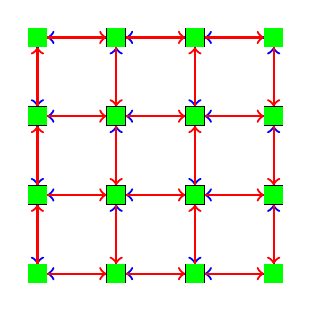
\begin{tikzpicture}
    \node[draw] (x11) at (0,0) {};
    \node[draw] (x12) at (0,1) {};
    \node[draw] (x13) at (0,2) {};
    \node[draw] (x14) at (0,3) {};
    \node[draw] (x21) at (1,0) {};
    \node[draw] (x22) at (1,1) {};
    \node[draw] (x23) at (1,2) {};
    \node[draw] (x24) at (1,3) {};
    \node[draw] (x31) at (2,0) {};
    \node[draw] (x32) at (2,1) {};
    \node[draw] (x33) at (2,2) {};
    \node[draw] (x34) at (2,3) {};
    \node[draw] (x41) at (3,0) {};
    \node[draw] (x42) at (3,1) {};
    \node[draw] (x43) at (3,2) {};
    \node[draw] (x44) at (3,3) {};
    % edges
    % vertical
    \draw (x11) to (x12);
    \draw (x12) to (x13);
    \draw (x13) to (x14);
    \draw (x21) to (x22);
    \draw (x22) to (x23);
    \draw (x23) to (x24);
    \draw (x31) to (x32);
    \draw (x32) to (x33);
    \draw (x33) to (x34);
    \draw (x41) to (x42);
    \draw (x42) to (x43);
    \draw (x43) to (x44);
    % horizontal
    \draw (x11) to (x21);
    \draw (x21) to (x31);
    \draw (x31) to (x41);
    \draw (x12) to (x22);
    \draw (x22) to (x32);
    \draw (x32) to (x42);
    \draw (x13) to (x23);
    \draw (x23) to (x33);
    \draw (x33) to (x43);
    \draw (x14) to (x24);
    \draw (x24) to (x34);
    \draw (x34) to (x44);
    % node x11
    \pause
    \node[green,fill] at (x11) {};
    \pause
    \draw[blue,thick,<-] (x11) to (x12);
    \draw[blue,thick,<-] (x11) to (x21);
    \pause
    \draw[red,thick,->] (x11) to (x12);
    \draw[red,thick,->] (x11) to (x21);
    % node x12
    \pause
    \node[green,fill] at (x12) {};
    \pause
    \draw[blue,thick,<-] (x12) to (x13);
    \draw[blue,thick,<-] (x12) to (x22);
    \pause
    \draw[red,thick,->] (x12) to (x13);
    \draw[red,thick,->] (x12) to (x22);
    % node x13
    \pause
    \node[green,fill] at (x13) {};
    \pause
    \draw[blue,thick,<-] (x13) to (x14);
    \draw[blue,thick,<-] (x13) to (x23);
    \pause
    \draw[red,thick,->] (x13) to (x14);
    \draw[red,thick,->] (x13) to (x23);
    % node x14
    \pause
    \node[green,fill] at (x14) {};
    \pause
    \draw[blue,thick,<-] (x14) to (x24);
    \pause
    \draw[red,thick,->] (x14) to (x24);
    % node x24
    \pause
    \node[green,fill] at (x24) {};
    \pause
    \draw[blue,thick,<-] (x24) to (x34);
    \draw[blue,thick,<-] (x24) to (x23);
    \pause
    \draw[red,thick,->] (x24) to (x34);
    \draw[red,thick,->] (x24) to (x23);
    % node x23
    \pause
    \node[green,fill] at (x23) {};
    \pause
    \draw[blue,thick,<-] (x23) to (x33);
    \draw[blue,thick,<-] (x23) to (x22);
    \pause
    \draw[red,thick,->] (x23) to (x33);
    \draw[red,thick,->] (x23) to (x22);
    % node x22
    \pause
    \node[green,fill] at (x22) {};
    \pause
    \draw[blue,thick,<-] (x22) to (x32);
    \draw[blue,thick,<-] (x22) to (x21);
    \pause
    \draw[red,thick,->] (x22) to (x32);
    \draw[red,thick,->] (x22) to (x21);
    % node x21
    \pause
    \node[green,fill] at (x21) {};
    \pause
    \draw[blue,thick,<-] (x21) to (x31);
    \pause
    \draw[red,thick,->] (x21) to (x31);
    % node x31
    \pause
    \node[green,fill] at (x31) {};
    \pause
    \draw[blue,thick,<-] (x31) to (x41);
    \draw[blue,thick,<-] (x31) to (x32);
    \pause
    \draw[red,thick,->] (x31) to (x41);
    \draw[red,thick,->] (x31) to (x32);
    % node x32
    \pause
    \node[green,fill] at (x32) {};
    \pause
    \draw[blue,thick,<-] (x32) to (x42);
    \draw[blue,thick,<-] (x32) to (x33);
    \pause
    \draw[red,thick,->] (x32) to (x42);
    \draw[red,thick,->] (x32) to (x33);
    % node x33
    \pause
    \node[green,fill] at (x33) {};
    \pause
    \draw[blue,thick,<-] (x33) to (x43);
    \draw[blue,thick,<-] (x33) to (x34);
    \pause
    \draw[red,thick,->] (x33) to (x43);
    \draw[red,thick,->] (x33) to (x34);
    % node x34
    \pause
    \node[green,fill] at (x34) {};
    \pause
    \draw[blue,thick,<-] (x34) to (x44);
    \pause
    \draw[red,thick,->] (x34) to (x44);
    % node x44
    \pause
    \node[green,fill] at (x44) {};
    \pause
    \draw[blue,thick,<-] (x44) to (x43);
    \pause
    \draw[red,thick,->] (x44) to (x43);
    % node x43
    \pause
    \node[green,fill] at (x43) {};
    \pause
    \draw[blue,thick,<-] (x43) to (x42);
    \pause
    \draw[red,thick,->] (x43) to (x42);
    % node x42
    \pause
    \node[green,fill] at (x42) {};
    \pause
    \draw[blue,thick,<-] (x42) to (x41);
    \pause
    \draw[red,thick,->] (x42) to (x41);
    % node x41
    \pause
    \node[green,fill] at (x41) {};
\end{tikzpicture}
\end{center}
\end{example}
\end{minipage}
 \pause
\begin{minipage}[t]{0.39\textwidth}
    \textbf{Damping Factor $\alpha$:}
\begin{itemize}
    \item We have seen that damping, i.e.\ $\alpha < 1$, can be helpful for convergence of Algorithms~\ref{alg:asynchronous-spmp}~and~\ref{alg:synchronous-spmp}.
 \pause
    \item Which values to choose in Example~\ref{example:sequential-message-passing-schedule}?
    \begin{itemize}
 \pause
        \item \textcolor{blue}{$\rightarrow$}: $\alpha = 1$.
 \pause
        \item \textcolor{red}{$\rightarrow$}: $\alpha = \frac{1}{\abs{\text{outgoing messages}}}$.
    \end{itemize}
 \pause
    \item Intuition: If we send $l$ messages from a single factor, then having cumulative weights $>1$ would overshoot.
\end{itemize}
\end{minipage}
\end{frame}

\begin{frame}{Bethe Cluster Graph}
\begin{itemize}
    \item Which cluster graph to choose naturally?
\end{itemize}
\pause
    \begin{definition}
        \label{def:bethe-cluster-graph}
    Given a Gibbs distribution $\Phi$ its Bethe cluster graph is a bipartite graph with 
        each node corresponding to either a variable or a factor with corresponding scopes and
        edges corresponding to whether a variable is in the scope of a factor.
    \end{definition}
\pause
\begin{example}[Bethe Cluster Graph]
   Consider $\tilde{\Pb} = \phi_{ABC} \phi_{BCD} \phi_{BDF} \phi_{BE} \phi_{DE}$.
   Its Bethe cluster graph is
\begin{center}
\begin{tikzpicture}
    % potentials
   \pause
   \node[rand_var] at (0,0) (ABC) {$A,B,C$}; 
   \node[rand_var] at (2,0) (BCD) {$B,C,D$};
   \node[rand_var] at (4,0) (BDF) {$B,D,F$};
   \node[rand_var] at (6,0) (BE) {$B,E$};
   \node[rand_var] at (8,0) (DE) {$D,E$};
   % variables
   \pause
   \node[rand_var] at (0,-2) (A) {$A$};
   \node[rand_var] at (0+1*1.6,-2) (B) {$B$};
   \node[rand_var] at (0+2*1.6,-2) (C) {$C$};
   \node[rand_var] at (0+3*1.6,-2) (D) {$D$};
   \node[rand_var] at (0+4*1.6,-2) (E) {$E$};
   \node[rand_var] at (0+5*1.6,-2) (F) {$F$};
   % edges
   \pause
   \draw (A) -- (ABC);
   \draw (B) -- (ABC);
   \draw (B) -- (BCD);
   \draw (B) -- (BDF);
   \draw (B) -- (BE);
   \draw (C) -- (ABC);
   \draw (C) -- (BCD);
   \draw (D) -- (BCD);
   \draw (D) -- (BDF);
   \draw (D) -- (DE);
   \draw (E) -- (BE);
   \draw (E) -- (DE);
   \draw (F) -- (BDF);
\end{tikzpicture}
\end{center}
\end{example}
\begin{itemize}
    \pause \item Note the similarity to the factor graph!
    \pause \item Information between different factors flows only through variable nodes.
    \begin{itemize}
        \pause \item Discards interaction between multiple variables and leads to poorer approximation.
    \end{itemize}
\end{itemize}
\end{frame}

\begin{frame}{Beyond Bethe Cluster Graph}
    \begin{itemize}
        \item Introduce intermediate cluster nodes that contain variable subsets.
        \pause Information flowing between factor nodes now contains higher-order variable interaction.
    \end{itemize}
 \pause
    \begin{definition}[Generalized Cluster Graph]
        Let $\Phi$ be a Gibbs distribution. Then its generalized cluster graph contains nodes that correspond to factors and variables as well as nodes that correspond to subsets of scopes of the variables.
        Edges are present whenever a node contains a subset of the variables in the scope of a factor and there is no smaller such one.
    \end{definition}
 \pause
    \begin{example}
   Consider $\tilde{\Pb} = \phi_{ABC} \phi_{BCD} \phi_{BDF} \phi_{BE} \phi_{DE}$.
\begin{center}
\begin{tikzpicture}
    % potentials
   \pause
   \node[rand_var] at (0,0) (ABC) {$A,B,C$}; 
   \node[rand_var] at (2,0) (BCD) {$B,C,D$};
   \node[rand_var] at (4,0) (BDF) {$B,D,F$};
   \node[rand_var] at (6,0) (BE) {$B,E$};
   \node[rand_var] at (8,0) (DE) {$D,E$};
   % pairs of variables
   \node[rand_var] at (0,-1) (AB) {$A,B$};
   \node[rand_var] at (2,-1) (BC) {$B,C$};
   \node[rand_var] at (4,-1) (BD) {$B,D$};
   \node[rand_var] at (6,-1) (CD) {$C,D$};
   \node[rand_var] at (8,-1) (DF) {$D,F$};
   % variables
   \pause
   \node[rand_var] at (0,-2) (A) {$A$};
   \node[rand_var] at (0+1*1.6,-2) (B) {$B$};
   \node[rand_var] at (0+2*1.6,-2) (C) {$C$};
   \node[rand_var] at (0+3*1.6,-2) (D) {$D$};
   \node[rand_var] at (0+4*1.6,-2) (E) {$E$};
   \node[rand_var] at (0+5*1.6,-2) (F) {$F$};
   % edges to pairwise subsets
   \pause
    \draw (A) -- (AB);
    \draw (B) -- (AB);
    \draw (B) -- (BC);
    \draw (B) -- (BD);
    \draw[bend right=20] (B) to (BE);
    \draw (C) -- (BC);
    \draw (C) -- (CD);
    \draw (D) -- (BD);
    \draw (D) -- (CD);
    \draw (D) -- (DF);
    \draw[bend right=10] (D) to (DE);
    \draw (F) -- (DF);
    \draw[bend right=30] (E) to (BE);
    \draw (E) -- (DE);
   % pairwise subsets to factors 
   \pause
   \draw (AB) -- (ABC);
   \draw (BC) -- (ABC);
   \draw (BC) -- (BCD);
   \draw (BD) -- (BCD);
   \draw (BD) -- (BDF);
   \draw (CD) -- (BCD);
   \draw (DF) -- (BDF);
\end{tikzpicture}
\end{center}
\end{example}
    
\end{frame}

\subsubsection{Excursion: Coding}

\begin{frame}{Excursion: Application to Codes}
    \begin{itemize}
        \item Assume we want to send $u_1,\ldots,u_k$ over a channel.
        \pause \item We encode the message as $x_1,\ldots, x_n$ (see below for possibilities how to do it).
        \pause \item After sending the encoded message, the receiver obtains $y_1,\ldots,y_n$.
        \begin{itemize}
            \pause \item The channel is noisy, and $x_i \neq y_i$ with some probability.
        \end{itemize}
        \pause \item One simple way to mitigate corruption: $x_{3 \cdot i} = x_{3 \cdot i + 1} = x_{3 \cdot i + 2} = u_i$ for all $i$.
        \begin{itemize}
        \item The receiver can then decode $\hat{u}_i$ as the majority vote over $y_{3\cdot i}$, $y_{3 \cdot i + 1}$ and $y_{3 \cdot i + 2}$.
        \end{itemize}
        \pause \item The \underline{bit error rate} is the probability that a bit is decoded incorrectly.
        \pause \item The \underline{rate of a code} is $k/n$, i.e.\ $1/3$ for the above code.
        \begin{itemize}
            \pause \item If the channel corrupts each bit with probability $p$, the bit error rate is $p^3 + 3p^2$ which is smaller than $p$ for $p$ small enough.
        \end{itemize}
        \pause \item Can we design better codes with higher rate and lower bit error rate?
    \end{itemize}
    \pause
    \begin{example}[Simple Parity Check Code]
        \label{example:parity-check-code}
            \begin{minipage}{0.49\textwidth}
            \begin{itemize}
                \item Original message: $u_1,\ldots,u_4$.
                \pause \item Encoding: 
                \begin{itemize}
                    \item $x_i = u_i$ for $i=1,\ldots,4$
                    \item $x_5 = u_1 + u_2 + u_3 \ mod\ 2$,
                    \item $x_6 = u_1 + u_2 + u_4 \ mod\ 2$,
                    \item $x_7 = u_2 + u_3 + u_4 \ mod\ 2$,
                \end{itemize}
            \pause \item Decoding?
            \end{itemize}
            \end{minipage}
            \begin{minipage}{0.49\textwidth}
                \begin{center}
            \begin{tikzpicture}[scale=0.7]
                \node[rand_var] at (0,0) (Y1) {$Y_1$};
                \node[rand_var] at (2,0) (Y2) {$Y_2$};
                \node[rand_var] at (4,0) (Y3) {$Y_3$};
                \node[rand_var] at (6,0) (Y4) {$Y_4$};
                \node[rand_var] at (0,-1) (X1) {$X_1$};
                \node[rand_var] at (2,-1) (X2) {$X_2$};
                \node[rand_var] at (4,-1) (X3) {$X_3$};
                \node[rand_var] at (6,-1) (X4) {$X_4$};
                \node[rand_var] at (0,-2) (U1) {$U_1$};
                \node[rand_var] at (2,-2) (U2) {$U_2$};
                \node[rand_var] at (4,-2) (U3) {$U_3$};
                \node[rand_var] at (6,-2) (U4) {$U_4$};
                \node[rand_var] at (1,-3) (X5) {$X_5$};
                \node[rand_var] at (3,-3) (X6) {$X_6$};
                \node[rand_var] at (5,-3) (X7) {$X_7$};
                \node[rand_var] at (1,-4) (Y5) {$Y_5$};
                \node[rand_var] at (3,-4) (Y6) {$Y_6$};
                \node[rand_var] at (5,-4) (Y7) {$Y_7$};
                % edges
                \draw[->] (X1) to (Y1);
                \draw[->] (X2) to (Y2);
                \draw[->] (X3) to (Y3);
                \draw[->] (X4) to (Y4);
                \draw[->] (U1) to (X1);
                \draw[->] (U2) to (X2);
                \draw[->] (U3) to (X3);
                \draw[->] (U4) to (X4);
                \draw[->] (U1) to (X5);
                \draw[->] (U1) to (X6);
                \draw[->] (U2) to (X5);
                \draw[->] (U2) to (X6);
                \draw[->] (U2) to (X7);
                \draw[->] (U3) to (X5);
                \draw[->] (U3) to (X7);
                \draw[->] (U4) to (X6);
                \draw[->] (U4) to (X7);
                \draw[->] (X5) to (Y5);
                \draw[->] (X6) to (Y6);
                \draw[->] (X7) to (Y7);
            \end{tikzpicture}
        \end{center}
            \end{minipage}
        \end{example}
    \end{frame}
    
    \begin{frame}{Excursion: Code Decoding Via Probabilistic Message Decoding}
        \begin{itemize}
            \pause \item \underline{Idea:} Reformulate message decoding as probabilistic inference task.
        \end{itemize}
        \textbf{Probabilistic Ansatz:}
        \begin{itemize}
            \item \underline{Prior} over message bits $U = (U_1,\ldots,U_k)$.
            \pause \item \underline{Encoder:} Function for converting $U$ to codeword $X = (X_1,\ldots,X_n)$.
            \pause \item \underline{Corruption:} Stochastic model for channel corruption $Y = (Y_1,\ldots,Y_n)$ given $X$.
            \pause \item \underline{Decoding:}  Find the most likely joint assignment of $U$ given the observed message bit $Y = y$, i.e.\ 
            \begin{equation}
                \argmax_{U} \Pb[U | Y = y]
            \end{equation}
        \end{itemize}
        \pause
        \hrule
        \begin{itemize}
            \item Clique tree message passing Algorithm~\ref{alg:calibration-sum-product-clique-tree} works for simple coding, like in Example~\ref{example:parity-check-code}.
            \pause \item Not applicable to codes with $n$ big enough and with large tree-width clique trees.
            \begin{itemize}
                \pause \item Use belief propagation instead!
                \pause \item A lot of the impetus on approximate inference came from this application.
            \end{itemize}
            \pause \item Nowadays used in hard drives, cellular communication, deep space communication etc.
        \end{itemize}
    \end{frame}

\subsubsection{Convex Belief Propagation}

\begin{frame}{Convex Belief Propagation}
Recall the Factored Free Energy:
\begin{equation}
        \tilde{F}[\tilde{\Pb}_{\Phi},Q] = \underbrace{\sum_{\phi \in \Phi} \E_{C_i \sim \beta_i}[\log(\psi_i)]}_{\text{linear}} \underbrace{+ \sum_{C_i} H_{\beta_i}(C_i)}_{\text{concave}} \underbrace{- \sum_{ij} H_{\mu_{ij}}(S_{ij})}_{\text{convex}}
\end{equation}
\begin{itemize}
\pause \item The Factored Free Energy is not a concave function of the beliefs $\beta_i$ and sepset beliefs $\mu_{ij}$.
\begin{itemize}
    \pause \item Stationary Points are local optimal in general.
\end{itemize}
\pause \item The negative entropy terms $H_{\mu_{ij}}$ for sepset beliefs destroy concavity.
\begin{itemize}
    \pause \item Idea: Reweight the sepset beliefs to make the overall objective concave.
\end{itemize}
\end{itemize}
\pause
\textbf{Ansatz:}
\begin{itemize}
    \item Introduce coefficients $\kappa_i, \kappa_{ij}$ for each entropy term to make the overall objective concave.
\end{itemize}
\pause
\begin{definition}[Counting Numbers, Weighted Approximate Entropy]
Introduce for each node and each edge in a cluster graph positive numbers $\kappa_i$, $\kappa_{ij}$, called counting numbers.
The weighted approximate entropy is    
\begin{equation}
        \tilde{H}^{\kappa}_Q(\mathcal{X}) =
          \sum_{C_i} \kappa_i H_{\beta_i}(C_i) - \sum_{ij} \kappa_{ij} H_{\mu_{ij}}(S_{ij})
\end{equation}
\end{definition}
\end{frame}

\begin{frame}{Factored Free Energy for Convex BP}
\textbf{Assumption:}
\begin{itemize}
    \item In the following we will assume a Bethe cluster graph (see Definition~\ref{def:bethe-cluster-graph}).
\end{itemize}
\pause
\hrule
The factored free energy for a Bethe cluster graph can be written as
\begin{equation}
    \label{eq:factored-free-energy-bethe-cluster-graph-orig}
        \tilde{F}[\tilde{\Pb}_{\Phi},Q] = \sum_{\phi \in \Phi} \E_{C_i \sim \beta_i}[\log(\psi_i)] + \sum_{\phi \in \Phi} H_{\beta_{\phi}}(C_\phi) + \sum_{i} H_{\beta_{i}}(X_i) - \sum_{(i,\phi): i \in \Scope(\phi)} H_{\mu_{i,\phi}}(X_i)\,.
\end{equation}
\pause
\begin{proposition}
For a calibrated set of beliefs the Bethe cluster graph with clusters $\{C_\phi : \phi \in \Phi\} \cup \{ X_i : X_i \in \mathcal{X}\}$, the factored free energy is equal to
\begin{equation}
    \label{eq:factored-free-energy-bethe-cluster-graph}
   \tilde{F}[\tilde{\Pb}_{\Phi},Q] = \sum_{\phi \in \Phi} \E_{C_i \sim \beta_i}[\log(\psi_i)] + \sum_{\phi \in \Phi} H_{\beta_{\phi}}(C_\phi) - \sum_{i} (d_i - 1) H_{\beta_{i}}(X_i)\,,
\end{equation}
where $d_i = \abs{\{ \phi \in \Phi : i \in \Scope[\phi]\}}$ is the number of factors that contain $X_i$.
\end{proposition}
\pause
\begin{proof}
    Immediate from the definition of factored free energy~\eqref{eq:factored-free-energy-bethe-cluster-graph-orig} and $H_{\beta_i}(X_i) = H_{\mu_{i,\phi}}(X_i)$ for calibrated beliefs.
\end{proof}
\end{frame}

\begin{frame}{Convex Counting Numbers}
\begin{itemize}
\item How to choose counting numbers $\kappa$ to make the weighted approximate entropy concave?
\end{itemize}
\pause
\begin{definition}[Convex Counting Numbers]
    Counting numbers $\kappa$ are called convex if there exist nonnegative numbers $\nu_{\phi},\nu_i$ and $\nu_{\phi,i}$ such that
    \begin{equation}
        \kappa_{\phi} = \nu_\phi + \sum_{i \in \Scope(\phi)} \nu_{\phi,i} \ \ \forall \phi \in \Phi,
        \quad \quad \quad \quad \quad
        \kappa_{i} = \nu_i - \sum_{i \in \Scope(\phi)} \nu_{\phi,i} \ \  \forall X_i \in \mathcal{X}\,.
    \end{equation}
\end{definition}
\pause
We can rewrite the entropy in the factored free energy function for Bethe cluster graphs~\eqref{eq:factored-free-energy-bethe-cluster-graph} as
\begin{multline}
    \label{eq:convex-weighted-entropy}
   \sum_{\phi} \kappa_{\phi} H_{\beta_{\phi}}(C_\phi) + \sum_{i} \kappa_{i} H_{\beta_{i}}(X_i) 
   = \\
   \sum_{\phi} \nu_{\phi} H_{\beta_{\phi}}(C_\phi) + \sum_{\phi,i : i \in \Scope[\phi]} \nu_{\phi,i} \left( H_{\beta_{\phi}}(C_{\phi}) - H_{\beta_{i}}(X_i) \right) + \sum_i \nu_{i} H_{\beta_{i}}(X_i)\,. 
\end{multline}
\pause
\begin{proposition}
    The weighted entropy~\eqref{eq:convex-weighted-entropy} is a concave function for any calibrated set of beliefs $Q$. 
\end{proposition}
\end{frame}

\begin{frame}{Weighted Entropy Concavity, Proof}
\begin{proof}
   The middle term in~\eqref{eq:convex-weighted-entropy} is a conditional entropy
   \begin{equation}
    \begin{aligned}
    & H_{\beta_{\phi}}(C_{\phi}) - H_{\beta_i}(X_i) \\
    \pause
    = &
    \sum_{C_{\phi}} \beta_{\phi}(C_{\phi}) \log(\beta_{\phi}(C_{\phi})) - \sum_{X_i} \beta_i(X_i) \log(\beta_i(X_i))\\
    \pause
    = &
    \sum_{C_{\phi}} \beta_{\phi}(C_{\phi}) \log(\frac{\beta_{\phi}(C_{\phi})}{\beta_i(X_i)}) \\
    \pause
    = &
    \sum_{X_i} \beta_i \sum_{C_{\phi} : {C_{\phi}}_i = X_i} \beta_{\phi}(C_{\phi} | X_i) \log(\beta_{\phi}(C_{\phi} | X_i)) \\
    \pause
    = &
    H_{\beta_{\phi}}(C_{\phi} | X_i)\,.
    \end{aligned}
   \end{equation}
   \pause
   Hence, all (conditional) entropies in~\eqref{eq:convex-weighted-entropy} have positive coefficients, making the overall function concave.
\end{proof}
\end{frame}

\begin{frame}{Convex Asynchronous Belief Propagation}
    \begin{algorithm}[H]
        \label{alg:convex-asynchronous-bp}
        \caption{Convex Asynchronous Belief Propagation}
        \KwInput{$\Phi$, $\kappa$}
        \tcp{Initialize messages}
        \For{$i,\phi : i \in \Scope[\phi]$}
        {
            $\delta_{\phi \rightarrow i}(X_i) \leftarrow 1$\;
            $\sigma_{i \rightarrow \phi}(C_{\phi}) \leftarrow 1$\;
        }
        \pause
        \tcp{Initialize counting numbers}
        $\hat{\nu}_i = \nu_i + \sum_{\phi : i \in \Scope[\phi]} \nu_{\phi}$ $\forall i$\;
        $\hat{\nu}_{i,\phi} = \nu_\phi + \nu_{i, \phi}$ $\forall i,\phi : i \in \Scope[\phi]$\;
        \pause
        \While{not converged}
        {
        \For{$i=1,\ldots,n$}
        {
        \pause
            \tcp{Compute incoming messages for $X_i$}
            \For{$\phi \in \Phi : i \in \Scope[\phi]$}
            {
                $\delta_{\phi \rightarrow i}(X_i) \leftarrow \sum_{C_{\phi} \backslash \{X_i\}} \left( 
                \phi(C_{\phi}) \prod_{j \in \Nb(\phi) \backslash \{i\}} \sigma_{j \rightarrow \phi}(C_{\phi})
               \right)^{1/\hat{\nu}_{i,\phi}} $\;
            }
        \pause
            \tcp{Compute beliefs for $X_i$}
            $\beta_i(X_i) \leftarrow \frac{1}{Z_{X_i}} \prod_{\phi \in \Phi : i \in \Scope[\phi]} \left( \delta_{\phi \rightarrow i}(X_i) \right)^{\hat{\nu}_{i,\phi}/\hat{\nu}_i}$\;
        \pause
            \tcp{Compute outgoing messages from $X_i$}
            \For{$\phi \in \Phi : i \in \Scope[\phi]$}
            {
                $\sigma_{i \rightarrow \phi}(C_{\phi}) \leftarrow 
                \left( \phi(C_{_{\phi}} \prod_{j \in \Scope[\phi] \backslash \{i\}} \sigma_{j \rightarrow \phi} (C_{\phi}) )\right)^{-\nu_{i,\phi}/\hat{\nu}_{i,\phi}}
                \left( \frac{\beta_i(X_i)}{\delta_{\phi \rightarrow i}(X_i)} \right)^{\nu_{\phi}}
                $\;
            }
        }
        }
    \end{algorithm}
\end{frame}

\begin{frame}{Convex Belief Propagation Discussion}
    \textbf{Discussion:}
    \begin{itemize}
        \item \underline{Advantages:}
        \begin{itemize}
            \pause \item Convex BP converges to the global optimum of the weighted free factored energy.
            \pause \item Many other algorithms from convex optimization can be applied.
        \end{itemize}
        \pause \item \underline{Disadvantages:}
        \begin{itemize}
            \pause \item The approximation to the free factored energy might not be good. Hence, solutions of convex BP might be worse than those of BP.
            \pause \item Standard BP often converges faster in practice.
        \end{itemize}
    \end{itemize}
    \textbf{Other considerations:}
\begin{itemize}
    \item How to choose counting numbers $\kappa$?
    \begin{itemize}
        \pause \item Search for $\kappa_{\phi}$ such that $\sum_{\phi} (\kappa_\phi - 1)^2$ is minimized. Counting numbers for factors are then as close as possible to $1$.
    \end{itemize}
\end{itemize}
\end{frame}


\subsubsection{Mean-Field Methods}
\begin{frame}{Mean-Field Methods Motivation}
\begin{itemize}
\item \underline{Belief Propagation:} Relative entropy $\rightarrow$ free energy $\rightarrow$ (convex) factored free energy.
\pause \item \underline{Mean-Field Methods:} Beliefs from $Q$ factorizing as $\Pb_{\Phi}$ $\rightarrow$ $Q$ factorizing as $\Phi' \subset \Phi$.
\end{itemize}
\pause \textbf{Formally:}
\begin{equation}
\label{eq:mean-field}
\max_{Q \in \mathcal{Q}} F[\tilde{\Pb},Q]
\end{equation}
\begin{minipage}{0.6\textwidth}
\begin{itemize}
\pause \item \underline{Exact Inference:} $\mathcal{Q} = \{\Pb : \Pb \text{ prob.\ distr.\ on } \mathcal{X}\}$.
\pause \item \underline{Mean-Field:} small $\mathcal{Q}$ of independent marginals, efficient, high approximation error.
\pause \item \underline{Structured Mean-Field:} complicated larger $\mathcal{Q}$ (e.g. low-treewidth subgraphs), less efficient, better approximation.
\end{itemize}
\end{minipage}
\begin{minipage}{0.39\textwidth}
    \begin{center}
    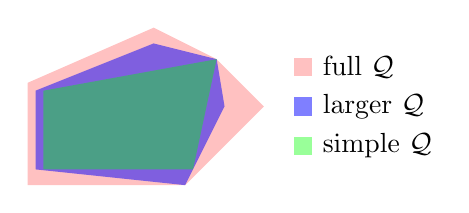
\begin{tikzpicture}
        \fill[red!30,opacity=0.8] (0,0) -- (2,0) -- (3,1) -- (2.4,1.6) -- (1.6,2) -- (0,1.3) -- cycle;
        \pause
        \fill[blue,opacity=0.5] (0.1,0.2) -- (2,0) -- (2.5,1) -- (2.4,1.6) -- (1.6,1.8) -- (0.1,1.2) -- cycle;
        \pause
        \fill[green,opacity=0.4] (0.2,0.2) -- (2.1,0.2) -- (2.4,1.6) -- (0.2,1.2) -- cycle;
        %legend
        \node at (3.5,1.5) [fill=red!30,opacity=0.8,label=right:full $\mathcal{Q}$] {};
        \node at (3.5,1) [fill=blue,opacity=0.5,label=right:larger $\mathcal{Q}$] {};
        \node at (3.5,0.5) [fill=green,opacity=0.4,label=right:simple $\mathcal{Q}$] {};
    \end{tikzpicture}
\end{center}
\end{minipage}
\pause
\begin{example}[Independent Marginals]
    The familiy of distributions with independent marginals are those distributions that can be written as
    \begin{equation}
    Q(\mathcal{X}) = \prod_i Q(X_i)\,.
    \end{equation}
\end{example}
\end{frame}

\begin{frame}{Mean-Field Energy Functional}
We will look into what the free energy is under independent marginals.
    \begin{itemize}
        \pause \item \underline{First term:}
        \begin{equation}
        \begin{aligned}
        \E_{Q}[\log(\phi)] 
        \pause = & \sum_{X_{\Scope[\phi]}} Q(X_{\Scope[\phi]}) \log(\phi(X_{\Scope[\phi]})) \\
        \pause = & \sum_{X_{\Scope[\phi]}} \left(\prod_{i \in \Scope[\phi]} Q(X_i) \right) \log(\phi(X_{\Scope[\phi]}))\,.
        \end{aligned}
        \end{equation}
        \pause \item \underline{Entropy term:}
        \begin{equation}
            \label{eq:entropy-marginal-distribution}
        \begin{aligned}
        H_Q(\mathcal{X}) 
        \pause = & - \sum_{X_{\Scope[\phi]}} Q(X_{\Scope}) \log(Q(X_{\Scope})) \\
        \pause = & - \sum_{X_{\Scope[\phi]}} \left(\prod_{i \in \Scope[\phi]} Q(X_i) \right) \log \left(\prod_{i \in \Scope[\phi]} Q(X_i)) \right) \\
        \pause = & - \sum_{i \in \Scope[\phi]} \underbrace{\sum_{X_{\Scope[\phi]} \backslash \{X_i\}} \left( \prod_{j \neq i} Q_j(X_j) \right)}_{=1} \sum_{X_i} Q(X_i) \log(Q(X_i)) \\
        %\pause = & - \sum_{i \in \Scope[\phi]} \sum_{X_i} Q(X_i) \log(Q(X_i)) \\
        \pause = & \sum_{i \in \Scope[\phi]} H_Q(X_i)
        \end{aligned}
        \end{equation}
        %\pause \item \underline{Factorization:} Both terms hence fully factorize according to the random variables and the topology of the network does not play a role.
    \end{itemize}
\end{frame}

\begin{frame}{Mean-Field Fixed Point}
The variational formulation for the marginal mean-field approximation is
\begin{equation}
    \label{eq:marginal-mean-field}
    %\begin{aligned}
    \max_{Q(X_1),\ldots,Q(X_n)}\ F[\tilde{\Pb}_{\Phi}, Q] 
    \quad
    \text{s.t. }  Q(X) = \prod_i Q(X_i), \quad
                  \sum_{X_i} Q(X_i) = 1\,.
    %\end{aligned}
\end{equation}
\pause
\begin{theorem}[Fixed Point of Marginal Mean-Field]
    \label{thm:local-maximal-marginal-mean-field}
    The distribution $Q(X_i)$ is a local maximum of~\eqref{eq:marginal-mean-field} given $\{Q(X_j)\}_{j \neq i}$ if and only if
    \begin{equation}
        \label{eq:marginal-mean-field-local-maximum}
        Q(X_i) = \frac{1}{Z_i} \exp\left(
             \sum_{\phi \in \Phi} \E_{\mathcal{X} \sim Q}[\log(\phi) | X_i] 
             \right)\,.
    \end{equation}
    where 
    \begin{equation}
        \E_{\mathcal{X} \sim Q}[\log(\phi) | X_i] 
        = 
        \sum_{X_{\Scope[\phi] \backslash \{X_i\}}} Q(X_{\Scope[\phi] \backslash \{X_i\}}) \log\left(\phi(X_{\Scope[\phi] \backslash \{X_i\}}, X_i) \right)
    \end{equation} 
    is the expected value of $\log(\phi)$ under the distribution $Q$ conditioned on $X_i$.
\end{theorem}
\pause
\begin{corollary}
    The distribution $Q$ is a stationary point of~\eqref{eq:marginal-mean-field} iff, for each $X_i$ equation~\eqref{eq:marginal-mean-field-local-maximum} holds.
\end{corollary}
\end{frame}

\begin{frame}{Mean-Field Fixed Point, Proof of Theorem~\ref{thm:local-maximal-marginal-mean-field}}
\begin{proof}
First, consider the restriction of the objective $F[\tilde{\Pb}_{\Phi},Q]$ to terms involving $Q(X_i)$:
\begin{equation}
    F_i[Q] 
    = \sum_{\phi \in \Phi} \E_{\mathcal{X} \sim Q}[\log(\phi)] + H_Q(X_i)\,.
    %= \sum_{\phi \in \Phi} \E_{\mathcal{X} \sim Q}[\log(\phi) | X_i] + H_Q(X_i)\,.
\end{equation}
\pause
To optimize $Q(X_i)$, define the Lagrangian
\begin{equation}
    L_i(Q,\lambda) = \sum_{\phi \in \Phi} \E_{\mathcal{X} \sim Q}[\log(\phi)] + H_Q(X_i) + \lambda (\sum_{X_i} Q(X_i) - 1)\,.
\end{equation}
\pause
Take derivatives with respect to $Q(X_i)$:
\begin{equation}
    \frac{\partial}{\partial Q(X_i)} L_i = \pause \sum_{\phi \in \Phi}
    \underbrace{\E_{X \sim Q}[ \log(\phi) | X_i]}_{= \frac{\partial \E_{X \sim Q}[\log(\phi)]}{\partial Q(X_i)}} \pause \underbrace{- \log(Q(X_i)) - 1}_{= \frac{\partial H_Q(X_i)}{\partial Q(X_i)}} \pause + \underbrace{\lambda}_{= \frac{\partial \lambda(\sum_{X_i} Q(X_i) - 1)}{\partial Q(X_i)}} = 0\,.
\end{equation}
\end{proof}
\end{frame}

\begin{frame}{Mean-Field Fixed Point, Proof of Theorem~\ref{thm:local-maximal-marginal-mean-field} cont.}
\begin{proof}
The derivative of the first term can be seen as follows:
\begin{equation}
    \begin{aligned}
    \frac{\partial}{\partial Q(X_i)} \E_{X \sim Q} [\log(\phi)] 
    \pause
    = & \frac{\partial}{\partial Q(X_i)} \sum_{X_{\Scope[\phi]}} \left( \prod_{i \in \Scope[\phi]} Q(X_i) \right) \log(\phi(X_{\Scope[\phi]})) \\
    \pause
    = & \sum_{X_{\Scope[\phi] \backslash \{i\}}} \left( \prod_{i \in \Scope[\phi] \backslash \{i\}} Q(X_i) \right) \log(\phi(X_{\Scope[\phi] \backslash \{i\}}, X_i)) \\
    \pause
    = & \E_{X \sim Q}[ \log(\phi) | X_i]
    \end{aligned}
\end{equation}
\pause
Derivative of entropy and Lagrange multiplier are standard.
\pause
Setting the derivative to $0$ and rearranging yields
\begin{equation}
    \log(Q(X_i)) = \lambda - 1 + \sum_{\phi \in \Phi} \E_{X \sim Q}[ \log(\phi) | X_i] \,.
\end{equation}
\pause
We take exponents and normalize.
\pause Since $\lambda$ is constant relative to $X_i$, it drops out in the normalization, so we obtain the result.
\end{proof}
\end{frame}

\begin{frame}{Mean-Field Algorithm}
\begin{algorithm}[H]
\label{alg:mean-field}
\caption{Mean-Field Algorithm}
\KwInput{Factors $\Phi$, Initial $Q_0$}
\pause
$Q \leftarrow Q_0$\;
\pause
$Unprocessed \leftarrow \mathcal{X}$\;
\pause
\While{$Unprocessed \neq \varnothing$}
{
    Choose $X_i$ from $Unprocessed$\;
    \pause
    $Q_{old}(X_i) \leftarrow Q(X_i)$\;
    \pause
    \For{$x_i \in Val(X_i)$}
    {
        $Q(x_i) \leftarrow \exp\left( \sum_{\phi \in \Phi : i \in \Scope[\phi]} \E_{X_{\Scope[\phi]} \backslash \{X_i\} \sim Q}[\log(\phi(X_{\Scope[\phi] \backslash \{X_i\}}), x_i)] \right)$\;
    }
    \pause
    Normalize $Q(X_i)$ to one\;
    \pause
    \If{$Q_{old}(X_i) \neq Q(X_i)$}
    {
        $Unprocessed \leftarrow Unprocessed \cup (\cup_{\phi \in \Phi: i \in \Scope[\phi]} \Scope[\phi])$\;
    }
    \pause
    $Unprocessed \leftarrow Unprocessed \backslash \{X_i\}$\;
}
return $Q$\;
\end{algorithm}
\begin{itemize}
\pause \item Each step in Algorithm~\ref{alg:mean-field} increases the free energy according to Theorem~\ref{thm:local-maximal-marginal-mean-field}.
\end{itemize}

    \pause
    \begin{theorem}[Mean-Field Convergence]
    The Mean-Field Algorithm~\ref{alg:mean-field} converges. The distribution $Q^*$ returned is a stationary point of $F[\tilde{\Pb},Q]$ subject to the constraint that $Q$ marginalizes.
    \end{theorem}
%\pause
%\begin{proof}
%    Each iteration of Algorithm~\ref{alg:mean-field} is monotonically nondecreasing.
%    \pause
%    Because the energy functional is bounded and the space of distributions is compact, there must exist a limit point $Q^*$.
%    \pause
%    Since the update equations are continuous, $Q^*$ must be a limit point.
%    \pause
%    At convergence, the fixed-point equations of Theorem~\ref{thm:local-maximal-marginal-mean-field} must hold for all variables in the domain.
%    \pause
%    As a consequence, the convergence point is a stationary point of the energy.
%\end{proof}
\end{frame}

\begin{frame}{Structured Mean-Field}
\begin{itemize}
\item \underline{Problem:} Marginal distributions might be too simplistic to capture the information contained in $\Pb_{\Phi}$.
\pause \item \underline{Idea:} \pause Use more expressive, but still tractable distribution.
\end{itemize}
\pause
\begin{example}
   \begin{tikzpicture}[scale=0.65,font=\scriptsize]
    \node at (1.5,3.75) {\small Original network};
   % nodes
   \node[rand_var] at (0,0) (x11) {$x_{11}$};
   \node[rand_var] at (1,0) (x12) {$x_{12}$};
   \node[rand_var] at (2,0) (x13) {$x_{13}$};
   \node[rand_var] at (3,0) (x14) {$x_{14}$};
   \node[rand_var] at (0,1) (x21) {$x_{21}$};
   \node[rand_var] at (1,1) (x22) {$x_{22}$};
   \node[rand_var] at (2,1) (x23) {$x_{23}$};
   \node[rand_var] at (3,1) (x24) {$x_{24}$};
   \node[rand_var] at (0,2) (x31) {$x_{31}$};
   \node[rand_var] at (1,2) (x32) {$x_{32}$};
   \node[rand_var] at (2,2) (x33) {$x_{33}$};
   \node[rand_var] at (3,2) (x34) {$x_{34}$};
   \node[rand_var] at (0,3) (x41) {$x_{41}$};
   \node[rand_var] at (1,3) (x42) {$x_{42}$};
   \node[rand_var] at (2,3) (x43) {$x_{43}$};
   \node[rand_var] at (3,3) (x44) {$x_{44}$};
   % edges
   % horizontal
   \draw (x11) -- (x12);
   \draw (x12) -- (x13);
   \draw (x13) -- (x14);
   \draw (x21) -- (x22);
   \draw (x22) -- (x23);
   \draw (x23) -- (x24);
   \draw (x31) -- (x32);
   \draw (x32) -- (x33);
   \draw (x33) -- (x34);
   \draw (x41) -- (x42);
   \draw (x42) -- (x43);
   \draw (x43) -- (x44);
   % vertical
   \draw (x11) -- (x21);
   \draw (x21) -- (x31);
   \draw (x31) -- (x41);
   \draw (x12) -- (x22);
   \draw (x22) -- (x32);
   \draw (x32) -- (x42);
   \draw (x13) -- (x23);
   \draw (x23) -- (x33);
   \draw (x33) -- (x43);
   \draw (x14) -- (x24);
   \draw (x24) -- (x34);
   \draw (x34) -- (x44); 

   \pause
        \begin{scope}[xshift=5cm]
    \node at (1.5,3.75) {\small Approx.\ network 1};
   % nodes
   \node[rand_var] at (0,0) (x11) {$x_{11}$};
   \node[rand_var] at (1,0) (x12) {$x_{12}$};
   \node[rand_var] at (2,0) (x13) {$x_{13}$};
   \node[rand_var] at (3,0) (x14) {$x_{14}$};
   \node[rand_var] at (0,1) (x21) {$x_{21}$};
   \node[rand_var] at (1,1) (x22) {$x_{22}$};
   \node[rand_var] at (2,1) (x23) {$x_{23}$};
   \node[rand_var] at (3,1) (x24) {$x_{24}$};
   \node[rand_var] at (0,2) (x31) {$x_{31}$};
   \node[rand_var] at (1,2) (x32) {$x_{32}$};
   \node[rand_var] at (2,2) (x33) {$x_{33}$};
   \node[rand_var] at (3,2) (x34) {$x_{34}$};
   \node[rand_var] at (0,3) (x41) {$x_{41}$};
   \node[rand_var] at (1,3) (x42) {$x_{42}$};
   \node[rand_var] at (2,3) (x43) {$x_{43}$};
   \node[rand_var] at (3,3) (x44) {$x_{44}$};
   % edges
   % horizontal
   \draw (x11) -- (x12);
   \draw (x12) -- (x13);
   \draw (x13) -- (x14);
   \draw (x21) -- (x22);
   \draw (x22) -- (x23);
   \draw (x23) -- (x24);
   \draw (x31) -- (x32);
   \draw (x32) -- (x33);
   \draw (x33) -- (x34);
   \draw (x41) -- (x42);
   \draw (x42) -- (x43);
   \draw (x43) -- (x44);
        \end{scope}

        \pause
        \begin{scope}[xshift=10cm]
    \node at (1.5,3.75) {\small Approx.\ network 2};
   % nodes
   \node[rand_var] at (0,0) (x11) {$x_{11}$};
   \node[rand_var] at (1,0) (x12) {$x_{12}$};
   \node[rand_var] at (2,0) (x13) {$x_{13}$};
   \node[rand_var] at (3,0) (x14) {$x_{14}$};
   \node[rand_var] at (0,1) (x21) {$x_{21}$};
   \node[rand_var] at (1,1) (x22) {$x_{22}$};
   \node[rand_var] at (2,1) (x23) {$x_{23}$};
   \node[rand_var] at (3,1) (x24) {$x_{24}$};
   \node[rand_var] at (0,2) (x31) {$x_{31}$};
   \node[rand_var] at (1,2) (x32) {$x_{32}$};
   \node[rand_var] at (2,2) (x33) {$x_{33}$};
   \node[rand_var] at (3,2) (x34) {$x_{34}$};
   \node[rand_var] at (0,3) (x41) {$x_{41}$};
   \node[rand_var] at (1,3) (x42) {$x_{42}$};
   \node[rand_var] at (2,3) (x43) {$x_{43}$};
   \node[rand_var] at (3,3) (x44) {$x_{44}$};
   % edges 
   % vertical
   \draw (x11) -- (x21);
   \draw (x21) -- (x31);
   \draw (x31) -- (x41);
   \draw (x12) -- (x22);
   \draw (x22) -- (x32);
   \draw (x32) -- (x42);
   \draw (x13) -- (x23);
   \draw (x23) -- (x33);
   \draw (x33) -- (x43);
   \draw (x14) -- (x24);
   \draw (x24) -- (x34);
   \draw (x34) -- (x44); 
        \end{scope}
   
\pause
        \begin{scope}[xshift=15cm]
    \node at (1.5,3.75) {\small Approx.\ network 3};
   % nodes
   \node[rand_var] at (0,0) (x11) {$x_{11}$};
   \node[rand_var] at (1,0) (x12) {$x_{12}$};
   \node[rand_var] at (2,0) (x13) {$x_{13}$};
   \node[rand_var] at (3,0) (x14) {$x_{14}$};
   \node[rand_var] at (0,1) (x21) {$x_{21}$};
   \node[rand_var] at (1,1) (x22) {$x_{22}$};
   \node[rand_var] at (2,1) (x23) {$x_{23}$};
   \node[rand_var] at (3,1) (x24) {$x_{24}$};
   \node[rand_var] at (0,2) (x31) {$x_{31}$};
   \node[rand_var] at (1,2) (x32) {$x_{32}$};
   \node[rand_var] at (2,2) (x33) {$x_{33}$};
   \node[rand_var] at (3,2) (x34) {$x_{34}$};
   \node[rand_var] at (0,3) (x41) {$x_{41}$};
   \node[rand_var] at (1,3) (x42) {$x_{42}$};
   \node[rand_var] at (2,3) (x43) {$x_{43}$};
   \node[rand_var] at (3,3) (x44) {$x_{44}$};
   % edges
   % horizontal
   \draw (x11) -- (x12);
   \draw (x12) -- (x13);
   \draw (x13) -- (x14);
   \draw (x21) -- (x22);
   \draw (x22) -- (x23);
   \draw (x23) -- (x24);
   \draw (x31) -- (x32);
   \draw (x32) -- (x33);
   \draw (x33) -- (x34);
   \draw (x41) -- (x42);
   \draw (x42) -- (x43);
   \draw (x43) -- (x44);
   % some connecting between rows
   \draw (x12) -- (x22);
   \draw (x23) -- (x33);
   \draw (x31) -- (x41);
        \end{scope}
   \end{tikzpicture} 
\end{example}
\pause
\begin{definition}[Structured Mean-Field Distribution]
    Given a set of potential scopes 
        $\{C_j \subset \mathcal{X} : j = 1,\ldots,J\}$
    the structured mean-field distribution is
    \begin{equation}
        Q(\mathcal{X}) = \frac{1}{Z_Q} \prod_{j=1}^J \psi_j\,, \quad \text{ where } \Scope[\psi_j] = C_j\,.
    \end{equation}
\end{definition}
\end{frame}

\begin{frame}{Structured Mean-Field Distribution}
    \begin{itemize}
        \item For structured mean-field to be tractable, we first study how the entropy behaves.
    \end{itemize}
    \pause
    \begin{proposition}
        If $Q(\mathcal{X}) = \frac{1}{Z_Q} \prod_j \psi_j$ is a structured mean-field distribution, then
        \begin{equation}
            H_Q(\mathcal{X}) = - \sum_{j=1}^J \E_{C_j \sim Q}[\log(\psi_j(C_j))] + \log(Z_Q)\,.
        \end{equation}
    \end{proposition}
    \pause
    \begin{proof}
    \begin{equation}
        \begin{aligned}
            H_Q(\mathcal{X}) 
            \pause = & - \sum_{\mathcal{X}} Q(\mathcal{X}) \log(Q(\mathcal{X})) 
            \pause = - \sum_{\mathcal{X}} Q(\mathcal{X}) \log \left( \frac{1}{Z_Q} \prod_{j=1}^J \psi_j(C_j) \right) \\
            \pause = & - \sum_{\j=1}^J \sum_{\mathcal{X}} Q(\mathcal{X}) \log(\psi_j(C_j)) + \sum_{\mathcal{X}} Q(\mathcal{X}) \log(Z_Q) 
            \pause = - \sum_{\j=1}^J \E_{C_j \sim Q}[\log \psi_j(C_j)] + \log(Z_Q) \\
        \end{aligned}
    \end{equation}
    \end{proof}
    \pause
    \begin{itemize}
        \item If we can compute the partition function $Z_Q$, we will be able to evalute $H_Q$.
        \pause \item We can use exact methods from before for $Z_Q$ for low tree-width distributions.
    \end{itemize}
\end{frame}

\begin{frame}{Structured Mean-Field Stationary Points}
    \begin{itemize}
        \item The overall the free energy can be written as
        \begin{equation}
            F[\tilde{\Pb}_{\Phi},Q] = \sum_{\phi} \E_Q[\log(\phi)] - \sum_{j=1}^J \E_Q[\log(\psi_j)] + \log(Z_Q)\,.
        \end{equation}
    \end{itemize}
    \pause
    \begin{theorem}[Fixed Points of Structured Mean-Field]
       If $Q(\mathcal{X}) = \frac{1}{Z_Q} \prod_j \psi_j$, then $Q$ is a stationary point of $F[\tilde{\Pb}_{\Phi},Q]$ if and only if 
       \begin{equation}
        \psi_j(C_j) \propto \exp \left(
            \E_Q[\log(\tilde{\Pb}_{\Phi} | C_j)] - \sum_{k \neq i} \E_Q[\log(\psi_k) | C_j] - F[\tilde{\Pb}_{\Phi}, Q]
            \right)\,.
       \end{equation}
    \end{theorem}
    \pause
    \begin{proof}
    Algebraic manipulations similar to the marginal mean-field case.
    \end{proof}
    \begin{itemize}
        \pause \item  The last term $F[\tilde{\Pb}_{\Phi},Q]$ above is independent of the state $C_j$.
        Hence, we can absorb this term into the normalization and ignore it.
    \end{itemize}
    \pause
    \begin{corollary}
       $Q(\mathcal{X}) = \frac{1}{Z_Q} \prod\limits_j \psi_j$ is stat.\ point of $F[\tilde{\Pb}_{\Phi},Q]$ iff 
        $\psi_j(C_j) \propto \exp (
            \E_Q[\log(\tilde{\Pb}_{\Phi} | C_j)] - \sum\limits_{k \neq i} \E_Q[\log(\psi_k) | C_j] 
            )$
    \end{corollary}
\end{frame}

\begin{frame}{Optimizing Structured Mean-Field}
In order to optimize $F[\tilde{\Pb}_{\Phi},Q]$, similarly to Algorithm~\ref{alg:mean-field} we:
\begin{itemize}
    \pause \item Set $\psi_j(C_j) = \exp\left( \E_Q[\log(\tilde{\Pb}_{\Phi} | C_j)] - \sum_{k \neq i} \E_Q[\log(\psi_k) | C_j] \right)$ to the right-hand side of the fixed-point equation and normalize
    \begin{itemize}
        \pause \item The first term $\E_Q[\log(\tilde{\Pb}_{\Phi} | C_j)]$ is conditioned on $C_j$ and therefore does not depend on $\psi_j(C_j)$.
        \pause \item Same for the second term $\sum_{k \neq i} \E_Q[\log(\psi_k) | C_j]$.
    \end{itemize}
    \pause \item As for marginal mean-field, this increases the objective and leads to convergence.
    \pause \item The evaluation of the rhs.\ requires inference over the structured distribution.
    \begin{itemize}
        \pause \item Use the exact methods we have developed so far.
    \end{itemize}
    \pause \item We can simplify update steps by discarding irrelevant sub-terms.
\end{itemize}
\pause
\begin{theorem}
If $Q(\mathcal{X}) = \frac{1}{Z_Q} \prod_j \psi_j$, then $\psi_j$ is locally optimal only if
\begin{equation}
    \psi_j(C_j) \propto \exp \left(
        \sum_{\phi \in A_j} \E_{\mathcal{X} \sim Q} [ \log(\phi) | C_j] - \sum_{\psi_k \in B_j} \E_Q[\log(\psi_k) | C_j]
        \right)
\end{equation}
where 
\begin{equation}
    A_j = \{\phi \in \Phi : X_{\Scope[\phi]} \indep C_j \text{ for } Q\}, \quad
    B_j = \{\psi_k : C_k \indep C_j \text{ for } Q\} \backslash \{\psi_j\}\,.
\end{equation}
\end{theorem}
\begin{itemize}
    \pause \item In words, the parametrization of $\psi_j$ only depends on factors in $\tilde{\Pb}_{\Phi}$ and in $Q$ whose scopes are not independent of $C_j$.
\end{itemize}
\end{frame}

\subsubsection{Expectation Propagation}
\begin{frame}{Factorized Messages Motivation}

\begin{itemize}
\item \underline{Belief Propagation:} Relax clique tree to cluster graph.
\pause \item \underline{Expectation Propagation:} Keep clique tree, relax message step.
\begin{itemize}
    \pause \item Approximate high-dimensional messages $\delta_{i \rightarrow j}$ by more compact representation.
    \pause \item Use product of marginals.
\end{itemize}
\end{itemize}

\pause
\begin{example}[$4 \times 4$ grid graph]
    \textbf{Clique Tree:}
    \begin{center}
    \begin{tikzpicture}[scale=0.8]
        % nodes
        \node[rand_var] at (0,0) (x11) {$x_{11}$};
        \node[rand_var] at (1,0) (x12) {$x_{12}$};
        \node[rand_var] at (2,0) (x13) {$x_{13}$};
        \node[rand_var] at (3,0) (x14) {$x_{14}$};
        \node[rand_var] at (0,1) (x21) {$x_{21}$};
        \node[rand_var] at (1,1) (x22) {$x_{22}$};
        \node[rand_var] at (2,1) (x23) {$x_{23}$};
        \node[rand_var] at (3,1) (x24) {$x_{24}$};
        \node[rand_var] at (0,2) (x31) {$x_{31}$};
        \node[rand_var] at (1,2) (x32) {$x_{32}$};
        \node[rand_var] at (2,2) (x33) {$x_{33}$};
        \node[rand_var] at (3,2) (x34) {$x_{34}$};
        \node[rand_var] at (0,3) (x41) {$x_{41}$};
        \node[rand_var] at (1,3) (x42) {$x_{42}$};
        \node[rand_var] at (2,3) (x43) {$x_{43}$};
        \node[rand_var] at (3,3) (x44) {$x_{44}$};
        % edges
        % horizontal
        \draw (x11) -- (x12);
        \draw (x12) -- (x13);
        \draw (x13) -- (x14);
        \draw (x21) -- (x22);
        \draw (x22) -- (x23);
        \draw (x23) -- (x24);
        \draw (x31) -- (x32);
        \draw (x32) -- (x33);
        \draw (x33) -- (x34);
        \draw (x41) -- (x42);
        \draw (x42) -- (x43);
        \draw (x43) -- (x44);
        % vertical
        \draw (x11) -- (x21);
        \draw (x21) -- (x31);
        \draw (x31) -- (x41);
        \draw (x12) -- (x22);
        \draw (x22) -- (x32);
        \draw (x32) -- (x42);
        \draw (x13) -- (x23);
        \draw (x23) -- (x33);
        \draw (x33) -- (x43);
        \draw (x14) -- (x24);
        \draw (x24) -- (x34);
        \draw (x34) -- (x44);

        \pause
        \draw[->] (3.5,1.5) to (4.5,1.5);

        \begin{scope}[xshift=5cm]
        \node[rand_var] at (0,0) (x11) {$x_{11}$};
        \node[rand_var] at (0,1) (x21) {$x_{21}$};
        \node[rand_var] at (0,2) (x31) {$x_{31}$};
        \node[rand_var] at (0,3) (x41) {$x_{41}$};
        \draw (x11) -- (x21);
        \draw (x21) -- (x31);
        \draw (x31) -- (x41);
        \end{scope}

        \pause
        \begin{scope}[xshift=6.5cm]
        \node[rand_var] at (0,0) (x11) {$x_{11}$};
        \node[rand_var] at (0,1) (x21) {$x_{21}$};
        \node[rand_var] at (0,2) (x31) {$x_{31}$};
        \node[rand_var] at (0,3) (x41) {$x_{41}$};
        \node[rand_var] at (1,0) (x12) {$x_{12}$};
        \node[rand_var] at (1,1) (x22) {$x_{22}$};
        \node[rand_var] at (1,2) (x32) {$x_{32}$};
        \node[rand_var] at (1,3) (x42) {$x_{42}$};
        \draw (x11) -- (x12);
        \draw (x21) -- (x22);
        \draw (x31) -- (x32);
        \draw (x41) -- (x42);
        \draw (x12) -- (x22);
        \draw (x22) -- (x32);
        \draw (x32) -- (x42);
        \end{scope}

        \pause
        \begin{scope}[xshift=9cm]
        \node[rand_var] at (0,0) (x12) {$x_{12}$};
        \node[rand_var] at (0,1) (x22) {$x_{22}$};
        \node[rand_var] at (0,2) (x32) {$x_{32}$};
        \node[rand_var] at (0,3) (x42) {$x_{42}$};
        \node[rand_var] at (1,0) (x13) {$x_{13}$};
        \node[rand_var] at (1,1) (x23) {$x_{23}$};
        \node[rand_var] at (1,2) (x33) {$x_{33}$};
        \node[rand_var] at (1,3) (x43) {$x_{43}$};
        \draw (x12) -- (x13);
        \draw (x22) -- (x23);
        \draw (x32) -- (x33);
        \draw (x42) -- (x43);
        \draw (x13) -- (x23);
        \draw (x23) -- (x33);
        \draw (x33) -- (x43);
        \end{scope}

        \pause
        \begin{scope}[xshift=11.5cm]
        \node[rand_var] at (0,0) (x13) {$x_{13}$};
        \node[rand_var] at (0,1) (x23) {$x_{23}$};
        \node[rand_var] at (0,2) (x33) {$x_{33}$};
        \node[rand_var] at (0,3) (x43) {$x_{43}$};
        \node[rand_var] at (1,0) (x14) {$x_{14}$};
        \node[rand_var] at (1,1) (x24) {$x_{24}$};
        \node[rand_var] at (1,2) (x34) {$x_{34}$};
        \node[rand_var] at (1,3) (x44) {$x_{44}$};
        \draw (x13) -- (x14);
        \draw (x23) -- (x24);
        \draw (x33) -- (x34);
        \draw (x43) -- (x44);
        \draw (x14) -- (x24);
        \draw (x24) -- (x34);
        \draw (x34) -- (x44);
        \end{scope}
    \end{tikzpicture}
\end{center}
\pause
    \textbf{Message Factorization:}
    \begin{itemize}
        \item $\delta_{1 \rightarrow 2}(X_{11}, X_{21}, X_{31}, X_{41}) = \delta_{1 \rightarrow 2}(X_{11}) \cdot \delta_{1 \rightarrow 2}(X_{21}) \cdot \delta_{1 \rightarrow 2}(X_{31}) \delta_{1 \rightarrow 2}(X_{41})$.
        \pause \item $\delta_{2 \rightarrow 3}(X_{12}, X_{22}, X_{32}, X_{42}) = \delta_{2 \rightarrow 3}(X_{12}) \cdot \delta_{2 \rightarrow 3}(X_{22}) \cdot \delta_{2 \rightarrow 3}(X_{32}) \delta_{2 \rightarrow 3}(X_{42})$.
        \pause \item $\delta_{3 \rightarrow 4}(X_{13}, X_{23}, X_{33}, X_{43}) = \delta_{3 \rightarrow 4}(X_{13}) \cdot \delta_{1 \rightarrow 2}(X_{23}) \cdot \delta_{3 \rightarrow 4}(X_{33}) \delta_{3 \rightarrow 4}(X_{43})$.
    \end{itemize}
\end{example}
\begin{itemize}
    \pause \item Internal structure of the cliques important for being able to compute marginal messages!
\end{itemize}
\end{frame}

\begin{frame}{Excursion: Projections}
    \begin{itemize}
        \item \underline{Problem:} How to approximate full message by product of marginal messages?
        \pause \item \underline{Solution:} Project full message onto space of marginal messages
    \end{itemize}
\hrule
\pause 
\begin{minipage}{0.49\textwidth}
    \begin{itemize}
        \item \underline{Projection:} Given point $y$, find nearest element to it in some set $C$, i.e.\ $y^* = \argmin_{x \in C} d(x,y)$.
    \end{itemize}
    \end{minipage}
    \pause
\begin{minipage}{0.49\textwidth}
            \begin{center}
            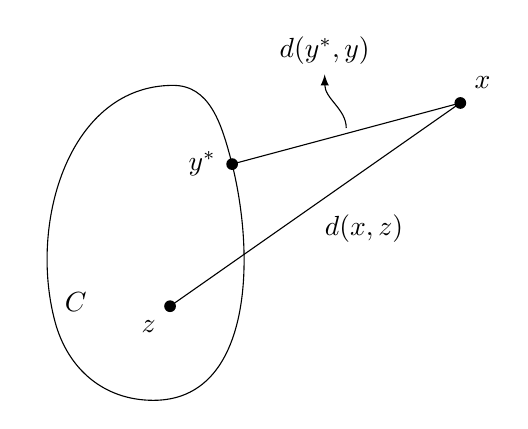
\begin{tikzpicture}[bullet/.style={circle,fill,inner sep=1.5pt,node contents={}}]
                \draw (0,0) node[bullet,label=left:$y^*$,alias=PC]  -- (15:3) coordinate[midway] (aux)
                   node[bullet,label=above right:$x$] -- ++ (-145:4.5) node[midway,below right]{$d(x,z)$}     node[bullet,label=below left:$z$];
                \draw (PC) to[out=105,in=0] ++ (-0.75,1) to[out=180,in=105] ++ (-1.5,-3)
                node[above right]{$C$} to[out=-75,in=180] ++ (1.25,-1) to[out=0,in=-75] cycle;
                \draw[shorten <=2pt,-latex] (aux) to[out=90,in=-90] ++ (110:0.8) node[above]{$d(y^*, y)$};
               \end{tikzpicture}
            \end{center}
    \end{minipage}
\pause
\hrule
\begin{itemize}
\item Projection set $C$ will be set of product messages. How to choose distance $d$?
\end{itemize}
\end{frame}
%
\begin{frame}{I- and M-Projection}
\begin{definition}[I-and M-Projection]
    Let $\Pb$ be a distribution and $\mathcal{Q}$ be a convex set of distributions.
    \begin{description}
        \pause \item[I-Projection,] also called information projection of $\Pb$ onto $\mathcal{Q}$, is defined as
        \begin{equation}
            Q^I = \argmin_{Q \in \mathcal{Q}} D(Q || \Pb)\,.
        \end{equation}
        \pause \item[M-Projection,] also called moment projection of $\Pb$ onto $\mathcal{Q}$, is defined as
        \begin{equation}
            Q^I = \argmin_{Q \in \mathcal{Q}} D(\Pb || Q)\,.
        \end{equation}
    \end{description}
\end{definition}
\pause
\textbf{Discussion:} \\
\begin{minipage}[h]{0.32\textwidth}
\begin{itemize}
    \item I-projection minimizes
    \begin{multline}
        D(Q || \Pb) = -H_Q(\mathcal{Q}) \\ + \E_Q[ -\log(\Pb)] \,.
    \end{multline}
    \begin{itemize}
    \pause \item First term: Penalty for low entropy.
    \pause \item Second term: Penalize large $Q$ for low $\Pb$.
\end{itemize}
\end{itemize}
\end{minipage}
\begin{minipage}[h]{0.32\textwidth}
\begin{itemize}
    \pause \item M-projection minimizes
        \begin{multline}
        D(\Pb || Q) = -H_{\Pb}(\mathcal{Q}) \\ + \E_{\Pb}[ -\log(Q)] \,.
        \end{multline}
    \begin{itemize}
    \pause \item First term: constant.
    \pause \item Second term: Penalize low $Q$ for high $\Pb$.
    \pause \item Try to cover support of $\Pb$.
        %$Q^M$ will prefer to have high values in regions that are probabily according to $\Pb$.
        %Simultaneously, there is a penalty to assigning low density to regions where $\Pb$ is not small. Its higher variance is a compromise for allowing to match the main mass of $\Pb$.
\end{itemize}
\end{itemize}
\end{minipage}
\pause
\begin{minipage}{0.32\textwidth}
%\pgfmathdeclarefunction{gauss}{2}{%
%  \pgfmathparse{1/(#2*sqrt(2*pi))*exp(-((x-#1)^2)/(2*#2^2))}%
%}
%\newcommand\gauss[2]{1/(#2*sqrt(2*pi))*exp(-((x-#1)^2)/(2*#2^2))} % Gauss function, parameters mu and sigma
\begin{center}
\begin{tikzpicture}[scale=0.5]
\begin{axis}[every axis plot post/.append style={
  mark=none,domain=-2:3,samples=50,smooth}, % All plots: from -2:2, 50 samples, smooth, no marks
  ticks=none,
  axis x line*=bottom, % no box around the plot, only x and y axis
  axis y line*=left, % the * suppresses the arrow tips
  enlargelimits=upper] % extend the axes a bit to the right and top
  \addplot {0.7*gauss(-0.5,0.5) + 0.3*gauss(1.3,1.0)};
  \addplot {gauss(-0.2,0.8)}; % I-projection
  \addplot {gauss(0,1.2)}; % M-projection
\end{axis}
% legend
\node at (5,5) [label=right:$\Pb$] {\textcolor{blue}{$-$}};
\pause
\node at (5,4) [label=right:$(\Pb)^I$] {\textcolor{red}{$-$}};
\pause
\node at (5,3) [label=right:$(\Pb)^M$] {\textcolor{black}{$-$}};
\end{tikzpicture}
\end{center}
%    \begin{center}
%    \includegraphics[width=0.98\textwidth]{img/I-M-Projections.png}
%    \end{center}
\end{minipage}
\end{frame}

\begin{frame}{Projection onto Independent Marginals}
\begin{theorem}
Let $\Pb$ be a distribution over $\mathcal{X}$ and $\mathcal{Q}$ be the family of independent marginals distributions. Then
\begin{equation}
    Q^M = \argmin_{Q \ \in \mathcal{Q}} D(\Pb || Q) = \Pb(X_1) \dots \Pb(X_n)\,.
\end{equation}
\end{theorem}
\pause
\begin{proof}
    \begin{equation}
        \begin{aligned}
            D(\Pb || Q) = &\E_{\Pb}[\log(\Pb(X_1,\ldots,X_n) - \log(Q(X_1,\ldots,X_n))] \\
            \pause = & \E_{\Pb}[\log(\Pb(X_1,\ldots,X_n)] - \sum_{i=1}^n \E_{\Pb}[\log(Q(X_i))] \\
            \pause = & \E_{\Pb}[\log(\frac{\Pb(X_1,\ldots,X_n)}{\Pb(X_1) \dots \Pb(X_n)}] + \sum_{i=1}^n \E_{\Pb}[\log(\frac{\Pb(X_i)}{Q(X_i)})] \\
            \pause = & D(\Pb || Q^M) + \sum_{i=1}^n D(\Pb(X_i) || Q(X_i)) \pause \geq D(\Pb || Q^M)
        \end{aligned}
    \end{equation}
    \pause
        The last step is due to non-negativity of $D$.
    \pause
        Equality holds only for $D(\Pb(X_i) || Q(X_i)) = 0$.%, i.e.\ $\Pb(X_i) = Q(X_i)$ for all $i$.
\end{proof}
%\end{frame}
%
%\begin{frame}{I-Projection onto Independent Marginals}
\begin{itemize}
    \pause \item What about $Q^I = 
    %\begin{equation}
        D(Q || \Pb) = - H_Q(\mathcal{X}) + \E_{Q}[\log(\Pb)]$?%\,.
    %\end{equation}
    \begin{itemize}
        \pause \item Entropy factorizes according to variables as seen in~\eqref{eq:entropy-marginal-distribution}.
        \pause \item Second term is not easy to handle, though.
    \end{itemize}
\end{itemize}
\end{frame}

\begin{frame}{Sum-Product Propagation}
\textbf{Idea:}
    Add M-projection after SP-Update in Algorithm~\ref{alg:calibration-sum-product-clique-tree}.

\begin{itemize}
    \pause \item Construct clique tree for $\Pb$ (might have large cliques now!).
    \pause \item Go over each sepset in up- and downstream order.
    \begin{itemize}
        \pause \item Compute message for variables in sepset.
        \pause \item Normalize to make it a distribution.
        \pause \item M-project onto marginal distribution.
    \end{itemize}
\end{itemize}
\pause
\begin{algorithm}[H]
   \caption{Sum-Product Propagation}
   \label{alg:calibration-sum-product-clique-tree}
    \KwInput{$\Phi$, root clique $C_r$, $T$}
    \tcp{Initialize Cliques}
    \For{$C \in T$}{
        $\psi_C \leftarrow \prod_{\phi: \xi[phi] = i} \phi$\;
    }
    \pause
    \tcp{Initialize Messages}
    \For{$ij \in E_T$}{
        $\delta_{i \rightarrow j}(X) = 1$, $\delta_{j \rightarrow i}(X) = 1$ $\forall X \in S_{ij}$
    }
    \pause
    \For{Up- and downstream pass}
    {
        Select $i \rightarrow j$ in correct order\;
        $\delta_{i \rightarrow j} \leftarrow \left(\frac{1}{Z} \sum_{C_i \setminus S_{ij}} \psi_{C_i} \cdot \prod_{k \in \Nb(i) \backslash \{j\}} \delta_{k \rightarrow i} \right)^M$\;
    }
\end{algorithm}
\begin{itemize}
    \pause \item Algorithm converges after one up- and downstream pass. \pause Why?
    \pause \item SP-update followed by M-projection can be computed by Clique-tree calibration Algorithm~\ref{alg:calibration-sum-product-clique-tree}.
\end{itemize}
\end{frame}

\begin{frame}{Belief-Update Expectation Propagation}
\textbf{Idea:} M-projection on beliefs. Two possibilities:
\begin{description}
    \pause \item[Sum-Product Propagation:] $\delta_{i \rightarrow j} \leftarrow \left( \frac{\beta_i}{\delta_{j \rightarrow i}} \right)^M$.
    \pause \item[Belief-Update Expectation Propagation:] $\delta_{i \rightarrow j} \leftarrow \frac{\left( \beta_i \right)^M}{\delta_{j \rightarrow i}}$.
\end{description}
\begin{itemize}
    \pause \item For exact sum-product update the above two operations are the same.
    \pause \item For expectation updates the two updates above are different.
    \pause \item Belief-Update takes into account in the projection step the current approximation of the beliefs including information coming from $j$. 
\end{itemize}
\pause
\begin{algorithm}[H]
   \caption{Sum-Product Propagation}
   \label{alg:calibration-sum-product-clique-tree}
    \KwInput{$\Phi$, root clique $C_r$, $T$}
    \tcp{Initialize Cliques}
    \For{$C \in T$}{
        $\psi_C \leftarrow \prod_{\phi: \xi[phi] = i} \phi$\;
    }
    \tcp{Initialize Messages}
    \For{$ij \in E_T$}{
        $\delta_{i \rightarrow j}(X) = 1$, $\delta_{j \rightarrow i}(X) = 1$ $\forall X \in S_{ij}$
    }
    \For{Up- and downstream pass}
    {
        Select $i \rightarrow j$ in correct order\;
        $\delta_{i \rightarrow j} \leftarrow \frac{\left(\frac{1}{Z} \sum_{C_i \setminus S_{ij}} \psi_{C_i} \cdot \prod_{k \in \Nb(i)} \delta_{k \rightarrow i}\right)^M}{\delta_{j \rightarrow i}}$.
    }
\end{algorithm}
\end{frame}

\begin{frame}{Variational Analysis of EP}
\textbf{Idea:} Link Belief-Update EP to maximizing $\tilde{F}[\tilde{\Pb}_{\Phi},Q]$.
\begin{itemize}
    \pause \item \underline{Problem:} We cannot enforce calibration, since we update beliefs only by marginal messages.
    \pause \item \underline{Solution:} Relax calibration requirements to expectation over variables, not sepsets.
\end{itemize}
\pause
\begin{equation}
    \label{eq:ep-optimization}
    \begin{aligned}
        \max_{Q}\ & \tilde{F}[\tilde{\Pb}_{\Phi}, Q] \\
        \text{s.t. } & \E_{S_{ij} \sim \mu_{ij}}[\mu_{ij} | X] = \E_{S_{ij} \sim \beta_j}[\beta_{i} | X] \quad \forall X \in \Scope[C_i] \cap \Scope[C_j] \\
        & \sum_{C_i} \beta_i(C_i) = 1  \quad \forall i,
        \quad \sum_{S_{ij}} \mu_{ij}(S_{ij}) = 1 \quad \forall ij, 
        \quad \beta, \mu \geq 0
    \end{aligned}
\end{equation}
\pause
\begin{theorem}[Stationary Points for Expectation Propagation]
    $Q$ is a stationary point for~\eqref{eq:ep-optimization} if and only if
    \begin{equation}
        \begin{aligned}
            \delta_{i \rightarrow j} & \propto \frac{\left(\frac{1}{Z} \sum_{C_i \setminus S_{ij}} \psi_{C_i} \cdot \prod_{k \in \Nb(i)} \delta_{k \rightarrow i}\right)^M}{\delta_{j \rightarrow i}} \\
            \beta_i & \propto \psi_i \cdot \prod_{j \in \Nb(i)} \delta_{j \rightarrow i} \\
            \mu_{ij} & \propto \delta_{j \rightarrow i} \delta_{i \rightarrow j}
        \end{aligned}
    \end{equation}
\end{theorem}
\end{frame}
%\begin{frame}{Factorized Messages}
%    \begin{itemize}
%        \item Recall that we want to compute approximations 
%        \begin{equation}
%    \delta_{i \rightarrow j}(S_{ij}) \approx \prod_{X \in S_{ij}} \delta_{i \rightarrow j}(X)\,.
%        \end{equation}
%        \pause \item How to measure distance of factorized message to full one?
%    \end{itemize}
%\end{frame}